\documentclass[11pt]{article}

\usepackage[T1]{fontenc}
\usepackage[utf8]{inputenc}
\usepackage[margin=1in]{geometry}
\usepackage{amsthm}
\usepackage[cmex10]{amsmath}
\usepackage{amssymb}
\usepackage{natbib}
\usepackage{tikz}
\usepackage{subcaption}
\usepackage{enumerate}
\usepackage{comment}
\usepackage[colorlinks,citecolor=blue,urlcolor=blue]{hyperref}

%\numberwithin{equation}{section}
\theoremstyle{plain}
\newtheorem{thm}{Theorem}%[section]
\newtheorem{lmm}{Lemma}%[section]
\newtheorem{prp}{Proposition}%[section]
\newtheorem{dfn}{Definition}%[section]
\newtheorem{example}{Example}%[section]
\newtheorem{crl}{Corollary}%[section]
\newtheorem{remark}{Remark}

\title{Asset Value and Securitization under Heterogeneous Beliefs}
\author{Oliver Pardo\thanks{Departamento de Administración, Pontificia Universidad Javeriana. Email: \href{mailto:pardoo@javeriana.edu.co}{pardoo@javeriana.edu.co}. I thank Jason Donaldson, Erik Eyster, Leonardo Felli, Francesco Nava, Daniel Osorio, Petr Postl, Balazs Szentes, and participants at the LSE Summer Seminar for comments and suggestions. All errors and omissions are my own.}}
\date{\today}

\begin{document}
\maketitle

\begin{abstract}
This paper studies how securitization affects asset prices and realized returns when investors hold heterogeneous beliefs. I extend the resale-option asset-pricing model of \cite{HarrisonKreps1978} by allowing the owner of a long-term asset to issue a finite set of asset-backed securities backed by its future cash flow. These securities are organized into tranches with different payment priorities. Because each tranche is priced by the investor most optimistic about that tranche, securitization weakly raises the value of the underlying asset. A strict increase requires that no belief about next-period asset prices first-order stochastically dominates all other beliefs. The same mechanism has ambiguous effects on realized returns: securitization can transfer low-return claims across agents. When one agent has the finest information partition, securitization may lower some agents' realized returns without raising anyone else's. The results provide a characterization of how belief disagreement shapes the impact of security design on asset prices and realized returns.

\end{abstract}

\noindent\textbf{JEL codes:} G12, G21, G24, D84.

\noindent\textbf{Keywords:} asset pricing; securitization; tranching; financial innovation; belief disagreement; bubbles.

\section{Introduction}

Can securitization raise the market value of an asset without changing its cash flow? This paper studies this question in an infinite-horizon asset-pricing model with heterogeneous beliefs and short-selling constraints. I compare a benchmark economy in which investors trade a risk-free bond and a long-term asset with economies in which the owner of the long-term asset can issue asset-backed securities (ABS) backed by its future cash flow. The central mechanism is that an investor who is not the most optimistic buyer of the whole asset may be the most optimistic buyer of a particular tranche.

In the resale-option model of \cite{HarrisonKreps1978}, the price of the whole asset reflects the valuation of the investor most optimistic about that asset. With securitization, the relevant object changes. Each tranche is priced by the investor most optimistic about the payoff range covered by that tranche. If perceived distributions over next-period asset prices cross, different tranches can be priced by different investors, and the sum of tranche prices can exceed the valuation of the whole asset by any single investor. Since ownership of the asset is necessary to issue the securities, the higher value of claims backed by the asset feeds back into the demand for the asset itself.

The paper formalizes this mechanism by allowing a finite number of risk-neutral investors to trade three types of assets in each period of a countably infinite sequence: i) an infinitely-supplied, risk-free, one-period bond, ii) a finitely-supplied, long-term asset that pays an uncertain dividend every period, and iii) securities backed by the latter. By issuing ABS, the owner of the long-term asset commits to transferring its future cash flow to the investors who buy the ABS. These securities have a waterfall payment structure: the most senior tranche promises a fixed amount unless the total cash flow from the underlying asset is below that amount; the next tranche is paid out of the cash flow left after the senior tranche is paid; and so on. The process of issuing ABS with this priority structure is referred to as \textit{tranching securitization}, or \textit{tranching} for short.

The equilibrium conditions follow from two assumptions. First, no naked positions are allowed: ownership of the long-term asset is necessary in order to issue ABS. Second, there is an exogenous limit on the short-selling of ABS. Since the long-term asset is in finite supply, these assumptions imply that the supply of ABS is finite as well. The fact that one-period bonds are in infinite supply implies that any investor can borrow as much as she wants at the market interest rate. Since there are no credit constraints, the equilibrium price of each ABS is given by the willingness to pay of whoever is most optimistic about the ABS's next payout. The paper shows that this equilibrium exists and is unique. If no short-selling constraints are assumed, the absence of credit constraints leads to an infinite supply of ABS and no equilibrium exists.

The first result is that tranching weakly raises the equilibrium price of the underlying asset. A strict increase requires that no perceived distribution over next-period asset prices first-order stochastically dominates all others. If one belief dominates, slicing the asset cannot create additional value. If perceived distributions cross, tranching can create claims that are valued most highly by different investors. As a result, the gap between the asset price and any perceived present value of dividends can widen.

The same mechanism has ambiguous effects on realized returns. Investors perceive their positions to break even, but their realized returns may differ once payoffs are evaluated under the objective transition probabilities. Following \cite{EysterPiccione2014}, I model beliefs as theories that may coarsen the state space. This allows a comparison between perceived break-even returns and the realized returns associated with the securities investors actually buy. Securitization can transfer low-return claims across investors: it may lower some investors' realized returns without raising anyone else's, but it can also make an investor's realized return less negative by shifting worse claims to someone else.

Relative to \cite{EysterPiccione2014}, the paper does not modify the behavioral foundation of incomplete and diverse perceptions. Instead, it asks how the possibility of designing securities backed by the long-term asset changes equilibrium prices and realized returns. This shift matters because the investor most optimistic about the whole asset need not be the investor most optimistic about each tranche. Relative to the literature on security design and collateral, the paper provides a simple characterization of when waterfall tranching can raise asset values under belief disagreement.

The mechanism is motivated by securitization before the 2007 financial crisis. Subprime mortgages were pooled into mortgage-backed securities (MBS), MBS were pooled into collateralized debt obligations (CDO), and CDO were further pooled into squared CDO. Instruments like MBS, CDO and squared CDO are ABS, securities whose payout is derived from and collateralized by underlying assets. The possibility of creating highly rated securities backed by subprime mortgages eased credit to subprime borrowers, fueling an increase in house prices \citep{Brunnermeier2009}.\footnote{For a historical account of security innovation, see \cite{Matthews1994}.} The purpose of the model is not to provide a full institutional account of that episode, but to isolate how belief disagreement and security design can interact to raise asset values.

This paper is organized as follows. The rest of this introduction presents a literature review. Section \ref{example} presents the motivating example that illustrates the setup and gives a hint of the main results. Section \ref{model} describes the general model, defines the equilibrium, and proves its existence and uniqueness. Section \ref{sec:eff} studies the effects of tranching securitization on the price of the underlying asset and on actual portfolio returns, and it comments on relaxing the waterfall payment constraint. Finally, Section \ref{sec:disc} presents some conclusions and suggestions for further research. Appendix \ref{sec:is} shows that multiple rounds of tranching are equivalent to a refinement of the initial tranching.

\subsection{Literature Review}

The paper belongs to the branch of asset-pricing literature under belief disagreement, of which \cite{Scheinkman2004} offer a survey. \cite{MilgromStokey1982} show that, if rational agents differ in information only but coincide on priors, there would be no trade. Because of this, numerous studies depart from the assumption of common priors. \cite{Miller1977} and \cite{HarrisonKreps1978} were pioneers in this regard. A non-exhaustive list of other studies on asset pricing with heterogeneous beliefs includes \cite{HarrisRavis1993}, \cite{Zapatero1998}, \cite{ChiarellaHe2001}, \cite{ScheinkmanXiong2003}, \cite{CaoOuYang2009}, \cite{XiongYan2010}, \cite{Geanakoplos2010}, \cite{HeXiong2010}, \cite{Cao2011}, and \cite{HansonSunderman2013}. Empirically, \cite{HongStein2007} advocate the use of heterogeneous beliefs to explain observed patterns in financial markets.

The paper also intersects with the literature on financial innovation and security design, of which \cite{DuffieRahi1995} offer a survey. Examples include \cite{Brock2009}, \cite{CheSethi2010}, \cite{FostelGeanakoplos2012}, \cite{Kubler2012}, and \cite{Simsek2013a, Simsek2013b}, which share with this paper the aim of studying the potentially destabilizing effects of financial innovation. \cite{Brock2009} shows that market selection among expectations can overshoot; \cite{Kubler2012} studies how market completion under heterogeneous beliefs can increase asset-price volatility; and \cite{Simsek2013b} shows that new financial assets can amplify speculative variance rather than merely improve risk sharing.

The works of \cite{FostelGeanakoplos2012} and \cite{Simsek2013a}, in particular, are closely related to this paper. Both works build on two-period general-equilibrium models where agents disagree about the dividend of a physical asset and collateral constraints discipline promises. This paper shares their prediction that tranching can increase asset prices, but it does so in a partial-equilibrium environment with an infinite horizon, any finite number of states, and any finite number of beliefs. The paper also goes beyond these works by studying the effect of securitization on the return each type of agent receives in the long run. Later work by \cite{GeanakoplosZame2014} and \cite{FostelGeanakoplos2016} is useful for positioning the paper in the broader collateral-equilibrium literature because it emphasizes how collateralizable promises can affect prices and investment even without changes in fundamentals.

Recent work on belief distortions, credit cycles, and financial crises also supports the paper's motivation. \cite{GennaioliShleiferVishny2012} connect financial innovation with neglected risks and fragility; \cite{BordaloGennaioliShleifer2018} provide a model of credit cycles driven by diagnostic expectations; \cite{BaronXiong2017} show that credit expansions predict crash risk that investors appear to neglect; and \cite{LopezSalidoSteinZakrajsek2017} document that elevated credit-market sentiment predicts subsequent reversals in credit conditions and economic activity. More recent work sharpens this point. \cite{GreenwoodHansonShleiferSorensen2022} show that rapid credit and asset-price growth predict financial crises; \cite{Maxted2024} studies how diagnostic expectations interact with financial intermediation to generate boom-bust investment cycles; \cite{KrishnamurthyLi2025} separate intermediation and sentiment mechanisms in crises; \cite{KrishnamurthyMuir2025} show that low pre-crisis spreads and rapid credit growth are typical before severe reversals; and \cite{BordaloGennaioliShleiferTerry2026} embed diagnostic expectations in a credit-cycle model with risky debt. These papers do not model waterfall tranching as in this paper, but they strengthen the empirical and behavioral case for studying how belief disagreement can raise asset prices and later damage returns.

Finally, the paper relates to security design and securitization. \cite{Garmaise2001} studies a firm designing a security to be auctioned among investors with statistically consistent but non-rational beliefs; \cite{DeMarzo2005} provides a canonical model of pooling and tranching; and \cite{BegleyPurnanandam2017} provide empirical evidence on the design of private-label RMBS deals. The contribution here is to characterize when waterfall tranching is issuer-optimal under belief disagreement and to show how the same mechanism affects agents' realized portfolio returns.

\section{Motivating example}\label{example}

Consider an environment where trade takes place in a countably infinite sequence of periods. Each period there is an infinitely supplied bond used as a numeraire that entitles a payoff $R>1$ next period. The bond can be traded for a finitely supplied asset that yields a random dividend $d$ every period. There are three possible states of the world, collected in the state space $X:=\{l,m,h\}$. The realizations of the dividend are such that $d(l) < d(m) < d(h)$. Securities backed by the long-term asset can be issued and traded.

There are two types of infinitely lived agents, $\mathcal{A}$  and $\mathcal{B}$. Both are risk-neutral. To keep the notation close to the general model, identify each type with the theory it uses.
A theory is a forecasting rule for the next-period state. In the block interpretation developed in Section \ref{model}, theory $\mathcal{A}$ has a single block, $\{l,m,h\}$, so it does not condition its forecasts on the current state. Theory $\mathcal{B}$ has three singleton blocks, $\{l\}$, $\{m\}$ and $\{h\}$, so it conditions its forecasts on the current state. For a theory $\mathcal{F} \in \{\mathcal{A},\mathcal{B}\}$, $Q_{\mathcal{F}}(x,y)$ is the probability, according to $\mathcal{F}$, of moving from current state $x$ to next-period state $y$. In every state, theory $\mathcal{A}$ assigns probability $1/3$ to each state next period. Meanwhile, theory $\mathcal{B}$ assigns probability $1-\epsilon$ to staying in the current state and is uniform otherwise:
\begin{align}
Q_{\mathcal{A}}(x,y) &= \frac{1}{3} && \text{for all } x,y\in X, \label{eq:QAexample}\\
Q_{\mathcal{B}}(x,y) &=
\begin{cases}
1-\epsilon, & \text{if } y=x,\\
\epsilon/2, & \text{if } y\neq x,
\end{cases}
&& x,y\in X. \label{eq:QBexample}
\end{align}

Let $P(x,y)$ denote the objective transition probability from state $x$ to state $y$. Throughout the example, take $P=Q_{\mathcal{B}}$. Thus, theory $\mathcal{B}$ coincides with the true transition process, whereas theory $\mathcal{A}$ is statistically consistent but does not condition on the current state: both theories imply the same long-run frequency for the three states, with each state occurring one third of the time.

The disagreement may emerge because agents use different forecasting tools or do not use all available information. There are many motivations for heterogeneous beliefs, but all require at least some agents to depart from rational expectations: if information is used efficiently, the realizations of the stochastic process feed back into agents' beliefs. Implicitly, the model assumes that the learning process has stalled.


\subsection{Benchmark: A world without asset-backed securities} \label{benchmark}

In the benchmark scenario, there are no asset-backed securities. Because of limited short-selling, the market clears when the long-term asset's highest expected return matches the return of the short-term bond. Let $q^0:X\to\mathbb{R}_+$ be the underlying-asset price function in the benchmark. Notation is simplified by assuming that the asset price is \textit{cum-dividend} and that the declared dividend is to be paid next period.

Consider the state $x \in X$. When considering buying the long-term asset, both agents are willing to pay $d(x)/R$ plus the discounted asset price they expect for next period. For agent $\mathcal{A}$, the expected price of the long-term asset is $\frac{1}{3}\left(q^0(l)+q^0(m)+q^0(h)\right)$. For agent $\mathcal{B}$, the same expectation is close  to $q^0(x)$. If, as happens in equilibrium, $q^0(l)<q^0(m)<q^0(h)$, agent $\mathcal{A}$ buys the long-term asset in state $l$ whereas agent $\mathcal{B}$ buys it in state $h$. Ex-ante, it is not clear who will buy the asset in state $m$. Still, the solution to the price function $q^0$ when $\epsilon$ goes to zero is given by

\begin{eqnarray}
q^0(l) & = & \frac{d(l)+\frac{1}{3}\left(q^0(l)+q^0(m)+q^0(h)\right)}{R} \label{ql} \\
q^0(m) & = & \frac{ d(m) + \max \left\{ q^0(m), \frac{1}{3} \left( q^0(l)+q^0(m)+q^0(h)\right) \right\} } {R} \label{qm}\\
q^0(h) & = & \frac{d(h)+q^0(h)}{R} \label{qh}
\end{eqnarray}
\\
For instance, if $R=2$, $d(l)=0$, $d(m)=2$ and $d(h)=3$, then $q^0(l)=1$, $q^0(m)=2$ and $q^0(h)=3$.

To illustrate the conditions under which the introduction of ABS increases the long-term asset price, consider the perceived distributions regarding the asset price for the next period. Let $G_\mathcal{F}(t\mid x)$ be the probability that the next-period asset price is less than or equal to $t\in\mathbb{R}_+$, as perceived by theory $\mathcal{F} \in \{\mathcal{A},\mathcal{B}\}$ conditional on being in state $x\in X$. Figure \ref{fig:CDFs} illustrates these conditional distributions for each of the three states. In states $l$ and $h$, the distributions can be ranked according to first-order stochastic dominance, as one distribution always takes values no lower than the other. The agent whose beliefs first-order stochastically dominate those of the other will buy the asset. In state $m$, there is no stochastic dominance between $G_\mathcal{A}(\cdot\mid m)$ and $G_\mathcal{B}(\cdot\mid m)$. Still, whoever has highest expectation regarding the asset price will buy the asset. At state $m$, the perceived distributions cross at $q^0(m)$: for realizations $t<q^0(m)$, $G_\mathcal{B}(t\mid m)<G_\mathcal{A}(t\mid m)$, whereas for realizations $t>q^0(m)$, $G_\mathcal{A}(t\mid m)<G_\mathcal{B}(t\mid m)$. Thus, theory $\mathcal{B}$ is more optimistic about avoiding low price realizations, while theory $\mathcal{A}$ is more optimistic about the upper tail. This divergence is exploited by ``slicing'' the asset into two securities: one with a payout attached to realizations below $q^0(m)$ and the other with a payout attached to realizations above $q^0(m)$. This is illustrated in the next subsection.

\begin{figure}[h!]
\centering
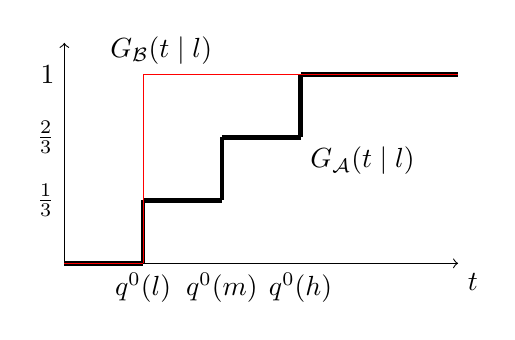
\begin{tikzpicture}[xscale=10,yscale=8]
\draw [<->] (0,0.35) -- (0,0) -- (0.5,0);
\node [below right] at (0.5,0) {$t$};
\draw [ultra thick]
(0.0,0.0) -- (0.1,0.0);
\draw [ultra thick]
(0.1,0.0) -- (0.1,0.1);
\draw [ultra thick]
(0.1,0.1) -- (0.2,0.1);
\draw [ultra thick]
(0.2,0.1) -- (0.2,0.2);
\draw [ultra thick]
(0.2,0.2) -- (0.3,0.2);
\draw [ultra thick]
(0.3,0.2) -- (0.3,0.3);
\draw [ultra thick]
(0.3,0.3) -- (0.5,0.3);
\node [below right] at (0.3,0.2) {$G_\mathcal{A}(t\mid l)$};
\node [left] at (0.0,0.1) {$\frac{1}{3}$};
\node [left] at (0.0,0.2) {$\frac{2}{3}$};
\node [left] at (0.0,0.3) {$1$};
\draw [red, domain=0:0.4] (0,0) -- (0.1,0.0);
\draw [red, domain=0:0.4] (0.1,0.0) -- (0.1,0.3);
\draw [red, domain=0:0.4] (0.1,0.3) -- (0.5,0.3);
\node [above left] at (0.2,0.3) {$G_\mathcal{B}(t\mid l)$};
\node [below] at (0.1,0) {$q^0(l)$};
\node [below] at (0.2,0) {$q^0(m)$};
\node [below] at (0.3,0) {$q^0(h)$};
\end{tikzpicture}

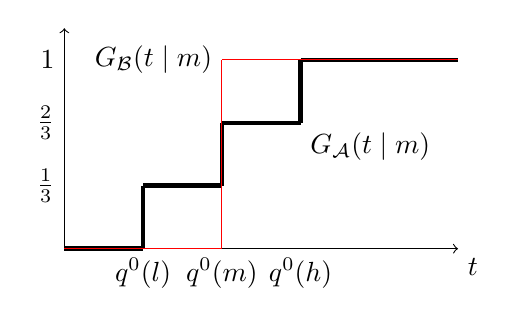
\begin{tikzpicture}[xscale=10,yscale=8]
\draw [<->] (0,0.35) -- (0,0) -- (0.5,0);
\node [below right] at (0.5,0) {$t$};
\draw [ultra thick]  (0.0,0.0) -- (0.1,0.0);
\draw [ultra thick] (0.1,0.0) -- (0.1,0.1);
\draw [ultra thick] (0.1,0.1) -- (0.2,0.1);
\draw [ultra thick] (0.2,0.1) -- (0.2,0.2);
\draw [ultra thick] (0.2,0.2) -- (0.3,0.2);
\draw [ultra thick] (0.3,0.2) -- (0.3,0.3);
\draw [ultra thick] (0.3,0.3) -- (0.5,0.3);
\node [below right] at (0.3,0.2) {$G_\mathcal{A}(t\mid m)$};
\node [left] at (0.0,0.1) {$\frac{1}{3}$};
\node [left] at (0.0,0.2) {$\frac{2}{3}$};
\node [left] at (0.0,0.3) {$1$};
\draw [red, domain=0:0.4] (0,0) -- (0.2,0.0);
\draw [red, domain=0:0.4] (0.2,0.0) -- (0.2,0.3);
\draw [red, domain=0:0.4] (0.2,0.3) -- (0.5,0.3);
\node [left] at (0.2,0.3) {$G_\mathcal{B}(t\mid m)$};
\node [below] at (0.1,0) {$q^0(l)$};
\node [below] at (0.2,0) {$q^0(m)$};
\node [below] at (0.3,0) {$q^0(h)$};
\end{tikzpicture}

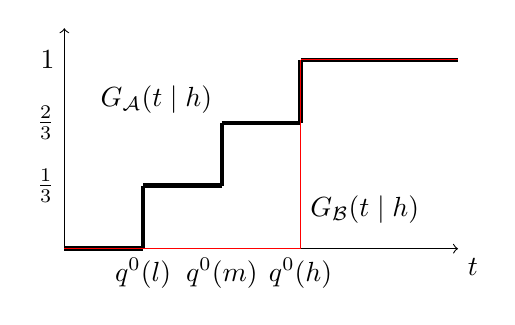
\begin{tikzpicture}[xscale=10,yscale=8]
\draw [<->] (0,0.35) -- (0,0) -- (0.5,0);
\node [below right] at (0.5,0) {$t$};
\draw [ultra thick] (0.0,0.0) -- (0.1,0.0);
\draw [ultra thick] (0.1,0.0) -- (0.1,0.1);
\draw [ultra thick] (0.1,0.1) -- (0.2,0.1);
\draw [ultra thick] (0.2,0.1) -- (0.2,0.2);
\draw [ultra thick] (0.2,0.2) -- (0.3,0.2);
\draw [ultra thick] (0.3,0.2) -- (0.3,0.3);
\draw [ultra thick] (0.3,0.3) -- (0.5,0.3);
\node [above left] at (0.2,0.2) {$G_\mathcal{A}(t\mid h)$};
\node [left] at (0.0,0.1) {$\frac{1}{3}$};
\node [left] at (0.0,0.2) {$\frac{2}{3}$};
\node [left] at (0.0,0.3) {$1$};
\draw [red, domain=0:0.4] (0,0) -- (0.3,0.0);
\draw [red, domain=0:0.4] (0.3,0.0) -- (0.3,0.3);
\draw [red, domain=0:0.4] (0.3,0.3) -- (0.5,0.3);
\node [below right] at (0.3,0.1) {$G_\mathcal{B}(t\mid h)$};
\node [below] at (0.1,0) {$q^0(l)$};
\node [below] at (0.2,0) {$q^0(m)$};
\node [below] at (0.3,0) {$q^0(h)$};
\end{tikzpicture}
\caption{Perceived distributions on the asset price} \label{fig:CDFs}
\end{figure}


\subsection{A world with asset-backed securities}\label{securitized}

Assume now that any owner of the long-term asset can issue two kinds of ABS, each of which has a maturity of one period. The claims of the ABS add up to the realization of the payout of the long-term asset. Each ABS belongs to one of two tranches: the \textit{senior} tranche and the \textit{junior} tranche. Let $q^1:X\to\mathbb{R}_+$ be the underlying-asset price function when these two kinds of ABS are issued. The ABS in the senior tranche guarantees a payoff $q^1(m)$ for next period unless the state becomes $l$, in which case it pays $q^1(l)$. The payoff from the junior tranche is $q^1(h)-q^1(m)$ if the realized state is $h$ and $0$ otherwise. In short, if $\phi_s$ and $\phi_j$ denote the payoff functions from senior and junior tranches, then

\begin{align}
\phi_s(t) & =  t - (t-q^1(m))^+, \label{spayoff} \\
\phi_j(t) & =  (t-q^1(m))^+, \label{epayoff}
\end{align}
\begin{figure}[h]
\centering
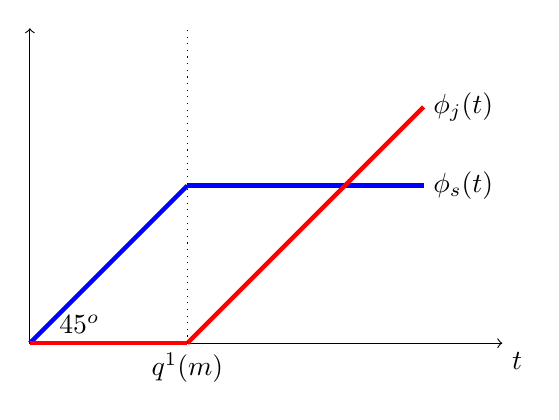
\begin{tikzpicture}[xscale=10,yscale=10]
\draw [<->] (0,0.4) -- (0,0) -- (0.6,0);
\node [below right] at (0.6,0) {$t$};
\draw [blue, ultra thick, domain=0:0.4] (0,0) -- (0.2,0.2);
\draw [blue, ultra thick, domain=0:0.4] (0.2,0.2) -- (0.5,0.2);
\node [right] at (0.5,0.2) {$\phi_s(t)$};
\draw [red, ultra thick, domain=0:0.4] (0,0) -- (0.2,0);
\draw [red, ultra thick, domain=0:0.4] (0.2,0) -- (0.5,0.3);
\node [right] at (0.5,0.3) {$\phi_j(t)$};
\draw [dotted] (0.2,0) -- (0.2,0.4);
\node [below] at (0.2,0) {$q^1(m)$};
\node [above right] at (0.025,0) {$45^{o}$};
\end{tikzpicture}
\caption{Payoff functions from senior and junior tranches}
\label{fig1:se}
\end{figure}

Figure \ref{fig1:se} plots the payoff from each tranche as a function of the cum-dividend price of the underlying asset. Note that i) owning the junior tranche is the same as holding a one-period call option on the underlying asset with strike price $q^1(m)$, and ii) owning the senior tranche is equivalent to owning the underlying asset together with a one-period written put option with strike price $q^1(m)$. In this particular example, the size of each tranche is given by $q^1(m)$. Such a threshold is known as an \textit{attachment point}.

On an alternative interpretation, the buyer of the junior tranche becomes the owner of the asset, but has a debt liability to the buyer of the senior tranche and is using the underlying asset as collateral. In this example, the junior buyer promises to pay $q^1(m)$ to the senior buyer in the next period. However, if the value of the collateral is $q^1(l)$, the junior buyer defaults and the senior buyer seizes the collateral.

Given the assumption about the existence of an exogenous constraint on short-selling, the price of each ABS is given by the willingness to pay from whoever is most optimistic about the payout of the ABS next period, discounted by the interest rate. To start with, assume $q^1(l)<q^1(m)<q^1(h)$. At state $m$, agent $\mathcal{B}$ expects a payoff close to $q^1(m)$ from the senior tranche, while agent $\mathcal{A}$ expects $\frac{2}{3}q^1(m)+\frac{1}{3}q^1(l)$. Hence, the senior tranche will be bought by agent $\mathcal{B}$. Meanwhile, agent $\mathcal{B}$ expects a  payoff close to zero from the junior tranche, while agent $\mathcal{A}$ expects $q^1(h)-q^1(m)$ with one-third probability. Hence agent $\mathcal{A}$ will buy the junior tranche. If $p_s(x)$ and $p_j(x)$ denote the prices of senior and junior tranches in state $x\in X$, then, as $\epsilon$ tends to zero,
\begin{eqnarray*}
p_s(m) & = & \frac{q^1(m)}{R} \\
p_j(m) & = & \frac{\frac{1}{3}\left(q^1(h)-q^1(m)\right)}{R}
\end{eqnarray*}

Since different agents might have claims on the same asset, the introduction of ABS can break the equivalence between any single expectation regarding the value of the underlying asset and the total value of the securities. To show this, note that at state $m$, the expectation on the asset price for next period is close to $q^1(m)$ for agent $\mathcal{B}$ and $\frac{1}{3}(q^1(l)+q^1(m)+q^1(h))$ for agent $\mathcal{A}$. Then
\begin{eqnarray*}
p_s(m) + p_j(m) & > &  \frac{q^1(m)}{R}  \\
p_s(m) + p_j(m) & > &  \frac{\frac{1}{3}\left(q^1(l)+q^1(m)+q^1(h)\right)}{R}
\end{eqnarray*}
which means that the payoff from selling the securities surpasses any expectation regarding the discounted price of the underlying asset.\footnote{See \cite{FostelGeanakoplos2012} for a similar result.}

The equilibrium price for the long-term asset is given by a non-arbitrage condition. Any agent could buy the long-term asset and sell the asset-backed securities derived from it. In equilibrium, the long-term asset cum-dividend price has to equal the discounted declared dividend plus the market value of the asset-backed securities:
\begin{equation} \label{eq:simarb}
q^1(x) = \frac{d(x)}{R} + p_s(x) + p_j(x)
\end{equation}
If the left-hand side of (\ref{eq:simarb}) were greater than the right-hand side, there would be no demand for the long-term asset. On the other hand, if the left-hand side were smaller than the right-hand side, demand would be infinite.

For states $l$ and $h$, the equilibrium conditions can be derived by identifying who buys the tranches at these states. At state $l$, the expectations of $\mathcal{A}$ on the payoff from any tranche are greater than those of $\mathcal{B}$. The opposite is true at state $h$. Hence both tranches are bought by $\mathcal{A}$ at state $l$ and both tranches are bought by $\mathcal{B}$ at state $h$. Adding up the tranche prices yields the discounted long-term asset price expected by whoever buys both tranches. Hence the price equations for $q^1(l)$ and $q^1(h)$ resemble equations (\ref{ql}) and (\ref{qh}).  The same is not true for $q^1(m)$, however, since at state $m$ each tranche is bought by different agents. In summary, the equilibrium price function $q^1$ is given by
\begin{eqnarray}
q^1(l) & = & \frac{d(l)+\frac{1}{3}\left(q^1(l)+q^1(m)+q^1(h)\right)}{R} \label{qpl}\\
q^1(m) & = & \frac{ d(m) +  q^1(m) + \frac{1}{3}(q^1(h)-q^1(m))} {R} \label{qpm} \\
q^1(h) & = & \frac{d(h)+q^1(h)}{R} \label{qph}
\end{eqnarray}

By comparing equation (\ref{qpm}) with equation (\ref{qm}), it can be seen that the introduction of ABS has increased the asset price at state $m$. This in turn increases the price at state $l$, since $\mathcal{A}$'s expectation at state $l$ is higher. Returning to the numerical example where $R=2$, $d(l)=0$, $d(m)=2$ and $d(h)=3$, the asset price increases by $\frac{1}{20}$ at state $l$ and by $\frac{1}{4}$ at state $m$. Thanks to the reselling opportunity, the introduction of ABS increases the asset price in states in which ABS appear to be innocuous.

Because $P=Q_{\mathcal{B}}$, theory $\mathcal{B}$ has rational expectations in this example and its actual excess return is zero both with and without ABS. Actual excess return refers to the one-period payoff from buying the asset or ABS, net of the payoff that the same expenditure would have obtained by buying the bond, averaged across states according to their long-run frequencies and evaluated under the objective transition $P$. Theory $\mathcal{A}$, instead, earns a negative excess return. In the numerical example, its excess return falls from $-\frac{1}{3}$ without ABS to $-\frac{13}{30}$ with ABS. Thus, in this example, securitization increases the price of the underlying asset while making the less sophisticated agent's realized return worse. This return effect is not general: Subsection \ref{sec:ep} later presents a case in which securitization makes an agent's excess return less negative, although it remains below zero. Appendix \ref{app:example-prices} reports the corresponding calculations.

\section{The Model}\label{model}

Consider an environment where trade takes place in each period of a countably infinite horizon. The assets traded in each period are of three kinds: 1) an infinitely supplied one-period bond used as a numeraire, 2) a single long-term asset that generates a random dividend every period, and 3) securities backed by the long-term asset.

\subsection{Dividends and interest rates}

The background structure of the model is given by an exogenous Markov process defined over a finite state-space $X$. The transition probability from state $x\in X$ to state $y\in X$ is given by $P(x,y)$, which is assumed to be strictly positive for every pair of states. This assumption is sufficient for the existence of a function $\mu:X\to(0,1)$ such that
\begin{equation}\label{eq:mu}
\mu(y)=\sum_{x\in X}P(x,y)\mu(x)
\end{equation}
for every $y\in X$. In the long-run, the world spends a fraction $\mu(x)$ of the time at state $x\in X$, regardless of the initial state.


\subsection{Beliefs}

All agents perceive that the state of the world evolves according to a Markov chain, but they may disagree on the transition probabilities. Each agent has a theory that represents her beliefs about the next-period state of the world. The finite set of theories in the market is represented by $\mathbf{F}$. The transition probability from state $x\in X$ to state $y\in X$, as perceived by theory $\mathcal{F}\in\mathbf{F}$, is denoted by $Q_\mathcal{F}(x,y)$.

A theory in $\mathbf{F}$ may be incomplete in the sense that it may be ignoring publicly available information. This idea is formalized by \cite{EysterPiccione2014} by defining an incomplete theory as a coarsening of the state-space. In this setup, every theory $\mathcal{F}\in\mathbf{F}$ is a partition of $X$. An element in $\mathcal{F}$ is known as a block of theory $\mathcal{F}$. If $x$ and $z$ are two different states in the same block of $\mathcal{F}$, then $Q_\mathcal{F}(x,y)=Q_\mathcal{F}(z,y)$ for all $y\in X$. This means that an agent using  theory $\mathcal{F}$ is ignoring the informational content of being at state $x$ rather than at state $z$.

Although it is assumed that theories may be incomplete, they are all supposed to achieve some degree of statistical consistency. In particular, all theories are assumed to agree in the long-run frequency of each state. Formally, let $\mathcal{F}(x)$ be the block in $\mathcal{F}$ that contains $x\in X$. All theories are assumed to satisfy:
\begin{equation} \label{eq:Q}
Q_{\mathcal{F}}\left(x,y\right)=\frac{\sum_{z\in \mathcal{F}\left(x\right)}P(z,y)\mu\left(z\right)}{\sum_{z\in \mathcal{F}\left(x\right)}\mu\left(z\right)}
\end{equation}
for all $y$ in $X$. By averaging across states, it follows that
\(\sum_{x\in X}Q_{\mathcal{F}}\left(x,y\right)\mu(x)=\mu(y)\),
meaning that there is no disagreement in the long-run frequency of any state.


If every block in a theory $\mathcal{F}$ is a singleton, it follows that $Q_\mathcal{F}=P$. In this case, $\mathcal{F}$ implies rational expectations. On the other side, if $\mathcal{F}=\left\{X\right\}$, then, $Q_{\mathcal{F}}\left(x,y\right)=\mu(y)$ for all $x$ and $y$ in $X$. This corresponds to the most naive theory, since its forecasts are not conditioned on the state.

The motivating example in Section \ref{example} fits this notation by using the state space $X=\{l,m,h\}$, a constant interest rate $R$, and $\mathbf{F}=\{\mathcal{A},\mathcal{B}\}$, with perceived transitions as in equations (\ref{eq:QAexample}) and (\ref{eq:QBexample}). Consistent with the assumption that $P=Q_{\mathcal{B}}$, theory $\mathcal{A}$ corresponds to the coarse partition $\{X\}$ and theory $\mathcal{B}$ corresponds to the singleton partition $\{\{l\},\{m\},\{h\}\}$.

One-period forward expectations play a pivotal role in the forthcoming analysis. To denote them, consider a random variable $s:X\to\mathbb{R}$. For any theory $\mathcal{F} \in \mathbf{F}$, the expectation regarding $s$ one period forward, conditional on being at state $x\in X$, is given by
\begin{equation}\label{eq:E}
E_{\mathcal{F}}\left(s\mid x\right):=\sum_{y\in X}s(y)Q_{\mathcal{F}}\left(x,y\right)
\end{equation}
Denote by $E\left(s\mid x\right)$ the expectation for the case where $Q_\mathcal{F}=P$. Equations (\ref{eq:mu}), (\ref{eq:E}) and (\ref{eq:Q}) imply that:
\begin{equation*}
\sum_{x\in X}E_{\mathcal{F}}\left(s\mid x\right)\mu(x)=\sum_{x\in X}E\left(s\mid x\right)\mu(x)
\end{equation*} for all $\mathcal{F}\in\mathbf{F}$. This means that the average one-period-ahead forecast of any theory matches the actual average of the random variable.

\subsection{Asset-backed securities}

The ownership of the long-term asset allows the possibility of obtaining liquidity (bonds) not only by reselling the asset but also by issuing and selling ABS. It is assumed that the ABS have a maturity of one period.
The security is a contract in which the owner of the long-term asset (the issuer) commits to transferring to the holder of the security (the investor) a non-negative amount of bonds next period. This amount depends on the realization of the asset price when payment is due. The securities are backed by the long-term asset in the sense that the net transfer from the issuer to all investors is always equal to the price of the underlying asset.

Formally, let $\mathcal{T}$ be a collection of non-overlapping intervals that partition the set $[0,\infty)$, which is the set of all conceivable realizations of the asset price. The partition $\mathcal{T}$ is known as a \textit{tranching} and an interval $\tau\in \mathcal{T}$ is known as a \textit{tranche}. Define $\underline{\tau}:=\inf(\tau)$ and $\overline{\tau}:=\sup(\tau)$. The payoff function
$\phi_\tau:\mathbb{R}_+\to\mathbb{R}_+$ from a security associated with tranche $\tau$ is given by
\begin{equation}\label{tpayoff}
\phi_\tau(t):=(t-\underline{\tau})^+-(t-\overline{\tau})^+
\end{equation}
where $t\in\mathbb{R}_+$
is a realization for the underlying asset price.

The point $\underline{\tau}$ is known as the \textit{attachment point}  of tranche $\tau$. This is because the tranche only starts to pay off when the realization for the asset price is above $\underline{\tau}$. Above $\overline{\tau}$, the payoff from tranche $\tau$ stalls at $\overline{\tau}-\underline{\tau}$ and the payoff from the next junior tranche (if any) detaches from 0. Figure \ref{fig:pay} illustrates the payoff function for a generic tranche.

\begin{figure}[h]
\centering
\begin{tikzpicture}[xscale=10,yscale=10]
\draw [<->] (0,0.4) -- (0,0) -- (0.6,0);
\node [below right] at (0.6,0) {$t$};
\node [right] at (0.5,0.2) {$\phi_\tau(t)$};
\draw [red, ultra thick, domain=0:0.4] (0,0) -- (0.1,0);
\draw [red, ultra thick, domain=0:0.4] (0.1,0) -- (0.3,0.2);
\draw [red, ultra thick, domain=0:0.4] (0.3,0.2) -- (0.5,0.2);
\draw [dotted] (0.1,0) -- (0.1,0.4);
\node [below] at (0.1,0) {$\underline{\tau}$};
\draw [dotted] (0.3,0) -- (0.3,0.4);
\node [below] at (0.3,0) {$\overline{\tau}$};
\node [above right] at (0.125,0) {$45^{o}$};
\end{tikzpicture}
\caption{Payoff function of a generic tranche $\tau$}
\label{fig:pay}
\end{figure}

The securities are backed by the long-term asset in the sense that they are \textit{budget balanced}: if $t$ is the realization of the asset price at the expiration date, the tranche payoffs add up to $t$:
\begin{equation*}
\sum_{\tau\in\mathcal{T}} \phi_\tau(t)=t
\end{equation*}
In addition, there is \textit{limited liability} for the issuer: $\phi_\tau(t) \geq 0$ for all $\tau\in\mathcal{T}$ and $t\in\mathbb{R}_+$.

In the example of Subsection \ref{benchmark}, there was no securitization so the tranching was given by $\mathcal{T}^0= \left\{ [0,\infty) \right\}$. In Subsection \ref{securitized}, there were only two tranches and the attachment point was calibrated so that the tranching was $\mathcal{T}^1=\{\tau^s,\tau^j\}$, where $\tau^s=[0,q^1(m))$ and $\tau^j=[q^1(m),\infty)$. Hence, the payoff functions in equations (\ref{spayoff}) and (\ref{epayoff}) are special cases of the generic expression in (\ref{tpayoff}).

\subsection{The market}

In each period, there is an infinitely-supplied bond used as a numeraire. The bond entitles a payoff $R(x)>1$ next period when the current state of the world is $x\in X$. The bond can be traded for a finitely-supplied asset that yields a random dividend $d(x)$ next period when the current state of the world is $x\in X$.


It is assumed that the short-selling of the ABS or the long-term asset is not possible. Alternatively, it can be assumed that there is an exogenous constraint on the short-selling of the ABS and of the long-term asset. Under this assumption, the price of any ABS will be given by the willingness to pay from whoever is most optimistic about the ABS future payout. Without any limit on the amount of ABS that can be short-sold, agents would be willing to take positions that would imply infinite bets on the future state of the world. If that were the case, there will be no equilibrium.


\subsection{Equilibrium} \label{sec:eq}

In equilibrium, the demand for the long-term asset and the demand for each security have to match their  respective supply. The exogenous limit on short-selling guarantees that this supply is finite.
For $x\in X$, let $p_\tau(x)$ be the price of the security associated with tranche $\tau\in\mathcal{T}$ and $q(x)$ be the price of the long-term asset.

\begin{dfn} \label{def:core}
For a given tranching $\mathcal{T}$, a waterfall equilibrium is a function $q:X\to\mathbb{R}_+$ and a collection of functions $p_\tau:X\to\mathbb{R}_+$ for $\tau\in\mathcal{T}$ such that
\begin{equation}\label{eqq}
q(x)=\frac{d(x)}{R\left(x\right)}+\sum_{\tau\in\mathcal{T}}p_\tau(x)
\end{equation}
and
\begin{equation}\label{eqp}
p_\tau(x)=\frac{\max_{\mathcal{F}\in\mathbf{F}}E_{\mathcal{F}}\left(\phi_\tau(q)\mid x\right)}{R(x)}
\end{equation}
for all $x\in X$.
\end{dfn}

Equation (\ref{eqq}) states that, in equilibrium, zero profits are made by buying the long-term asset and selling the securities derived from it. Equation (\ref{eqp}) states that the price of each security is given by the highest discounted expectation regarding the payoff from the corresponding tranche.

\subsection{Existence and uniqueness} \label{sec:extuni}

The existence and uniqueness of a waterfall equilibrium is proved by constructing the following object: For any tranching $\mathcal{T}$, define a mapping $\Psi_\mathcal{T}$ from the set of price functions $\mathbb{R}_+^X$ to itself. For $q\in\mathbb{R}_+^X$ and $x\in X$, the mapping is given by

\begin{equation} \label{eq:map}
\Psi_{\mathcal{T}}(q)(x)=\frac{d(x)+\sum_{\tau\in\mathcal{T}}\max_{\mathcal{F}\in\mathbf{F}}E_{\mathcal{F}}\left(\phi_\tau(q)\mid x\right)}{R\left(x\right)}
\end{equation}
By substituting equation (\ref{eqp}) into equation (\ref{eqq}), it follows that a long-term asset price function $q$ must be a fixed point of $\Psi_\mathcal{T}$ in order to be part of an equilibrium.

\begin{prp} \label{exu}
For every tranching $\mathcal{T}$, there is a unique waterfall equilibrium.
\end{prp}

\begin{proof}
The mapping $\Psi_{\mathcal{T}}$ has a unique fixed point since it satisfies Blackwell's sufficient conditions:
\begin{enumerate}
\item (Monotonicity) For all $q,q' \in \mathbb{R}_+^X$ such that $q(x)\leq q'(x)$ for all $x\in X$,
\begin{equation*}
\Psi_{\mathcal{T}}(q)(x) \leq \Psi_{\mathcal{T}}(q')(x)
\end{equation*}
for all $x\in X$.
\item (Discounting) For any $q \in \mathbb{R}_+^X$ and $c\geq0$,
\begin{equation*}
\Psi_{\mathcal{T}}(q+c)(x)\leq \Psi_{\mathcal{T}}(q)(x)+\left(\min_{y\in X}R\left(y\right)\right)^{-1}c
\end{equation*}
for all $x\in X$.
\end{enumerate}
\end{proof}

\section{The effects of tranching} \label{sec:eff}

This section studies the effect of tranching securitization, understood as the introduction of new ABS with a waterfall payment constraint, on the equilibrium price of the long-term asset. Formally, tranching securitization means a refinement of the existing tranching:
\begin{dfn} \label{def:tranching-sec}
An economy engages in tranching securitization if it switches from a tranching $\mathcal{T}$ to a tranching  $\mathcal{S}$, where $\mathcal{S}$ is a refinement of $\mathcal{T}$.
\end{dfn}
This means that agents who buy the long-term asset are able to sell a greater variety of tranches. Appendix \ref{sec:is} shows that this definition is equivalent to being able to issue new ABS backed by the existing ABS.

\subsection{Effect on asset prices}

Denote by $q_\mathcal{T}$ the waterfall equilibrium price for the long-term asset for tranching $\mathcal{T}$. Further securitization cannot decrease the price of the underlying asset:
\begin{lmm} \label{refine}
If $\mathcal{S}$ is a refinement of $\mathcal{T}$, then \begin{equation*}
q_{\mathcal{T}}(x) \leq q_{\mathcal{S}}(x)
\end{equation*}
for all $x\in X$
\end{lmm}
\textsc{Proof:} See Appendix.

Intuitively, there is no harm to the issuer from slicing the cash flow of the underlying asset into more tranches: if the issuer is lucky, investors who were outbid when the big tranches were issued will push harder when bidding for smaller tranches. At worst, investors will be indifferent.\footnote{It should be noted, though, that this result will hold even if the waterfall constraint is absent - see Subsection \ref{sec:cds}.}

It is worth comparing the benchmark scenario, where there is no tranching, with any scenario where there is some degree of tranching:

\begin{crl} \label{cor:eonben}
Define $q^0:=q_{\left\{[0,\infty)\right\}}$ as the price of the long-term asset in the absence of any tranching. Then, for any tranching $\mathcal{T}$,
\begin{equation} \label{eq:eonben}
q^0(x)\leq q_{\mathcal{T}}(x)
\end{equation}
for every $x\in X$.
\end{crl}

\begin{proof}
Since any tranching $\mathcal{T}$ is a refinement of $\left\{[0,\infty)\right\}$, inequality (\ref{eq:eonben}) follows from Lemma \ref{refine}.
\end{proof}

The function $q^0$ is a lower bound on asset prices in the sense that any tranching $\mathcal{T}$ cannot decrease the asset price below $q^0(x)$ at any $x\in X$. Intuitively, the price of the long-term asset without any tranching, $q^0(x)$, is given by the highest expectation on the cash flow coming from the whole asset. In contrast, the price of the long-term asset when there is some degree of tranching, $q_{\mathcal{T}}(x)$, is obtained by adding up the highest expectations on the cash flow coming from each tranche. The highest expectation on the cash flow from the whole asset cannot be higher than the sum of the highest expectations on the cash flow from each tranche.

Still, a satisfactory explanation for the issuing of ABS will have to show that it \textit{strictly} increases the asset price in at least one state. If this is the case, then it will be natural to assume that anyone who buys the long-term asset will issue ABS until the tranching stops increasing the asset value. A tranching is said to be \textit{issuer-optimal} if no other tranching can increase the asset price in any state:
\begin{dfn} \label{def:fse}
A tranching $\mathcal{T}$ is issuer-optimal if
\begin{equation*}
q_{\mathcal{S}}(x) \leq
q_{\mathcal{T}}(x)
\end{equation*}
for any tranching $\mathcal{S}$ and all $x\in X$.
\end{dfn}

In order to characterize the necessary and sufficient conditions for a tranching to be issuer-optimal, the following object is introduced: Let $I_A$ be the indicator function for event $A$. For $t\in\mathbb{R}_+$, define $G^\mathcal{T}_\mathcal{F}\left(t\mid x\right)$ as the probability at state $x$ that the asset price  next period is no higher than $t$, as perceived by theory $\mathcal{F}$ when the tranching is $\mathcal{T}$:
\begin{equation*}
G^\mathcal{T}_\mathcal{F}\left(t\mid x\right) := E_{\mathcal{F}}\left(I_{\left\{q_\mathcal{T}\leq t\right\}}\mid x\right)
\end{equation*}
\begin{prp} \label{mthm}
A tranching $\mathcal{T}$ is issuer-optimal if and only if, for each  $\tau\in\mathcal{T}$ and $x\in X$, there is a theory $\mathcal{G}\in\mathbf{F}$ such that
\begin{equation*}
G^{\mathcal{T}}_
{\mathcal{G}}
\left(t\mid x\right)
\leq
G^{\mathcal{T}}_
{\mathcal{F}}
\left(t\mid x\right)
\end{equation*}
for $d\phi_\tau$-almost every $t\in\tau$ and all $\mathcal{F}\in\mathbf{F}$.
\end{prp}
\textsc{Proof:} See Appendix.

Proposition \ref{mthm} states that a tranching is issuer-optimal if and only if for every state and every tranche, there is someone who is more optimistic than everyone else regarding the asset price not being below any realization in the tranche. If this is not the case, then there is a tranching that will increase the asset price in every state. This is because at some state there will be someone willing to outbid whoever is buying the current tranche whenever a smaller tranche is issued.

A natural question is whether the benchmark with no tranching is issuer-optimal. Denote by $G^0_{\mathcal{F}}(\cdot\mid x)$ the cumulative distribution function of the asset price for theory $\mathcal{F}$ when there is no tranching, i.e.,
\begin{equation*}
G^0_\mathcal{F}\left(t\mid x\right) := E_{\mathcal{F}}\left(I_{\left\{q^0\leq t\right\}}\mid x\right)
\end{equation*}
for $t\in\mathbb{R}_+$.
\begin{crl}
The tranching $\left\{[0,\infty)\right\}$
is issuer-optimal if and only if, for each $x\in X$, there is a theory $\mathcal{G}\in\mathbf{F}$ such that
$G^0_{\mathcal{G}}
\left(\cdot\mid x\right)$
first-order stochastically dominates
$G^0_{\mathcal{F}}
\left(\cdot\mid x\right)$
for all $\mathcal{F}\in\mathbf{F}$.
\end{crl}
\begin{proof}
Follows directly from Proposition \ref{mthm}.
\end{proof}
If there is only one theory in the market, the first-order stochastic dominance condition trivially holds. As expected, the benchmark without tranching is issuer-optimal if there is no belief disagreement.

As an example of a tranching that is not issuer-optimal, consider $\mathcal{T}^0=\left\{[0,\infty)\right\}$ in Subsection \ref{benchmark}: there is no first-order stochastic dominance between beliefs at state $m$, as illustrated by Figure \ref{fig:CDFs}. On the other hand, the tranching $\mathcal{T}^1=\left\{[0,q^1(m)),[q^1(m),\infty)\right\}$ in Subsection \ref{securitized} is issuer-optimal: for each tranche and each state there is always an agent whose conditional cumulative distribution of the asset price caps the other one along the realizations in the tranche.

Finally, it is worth remarking that whenever the introduction of ABS increases the asset price, the asset will be traded at a price higher than anyone thinks it is worth:

\begin{prp} \label{rem:worth}
If  $\left\{[0,\infty)\right\}$ is not issuer-optimal, then there is a tranching $\mathcal{T}$ in which the waterfall equilibrium $q_{\mathcal{T}}$ is such that
\begin{equation*}
q_{\mathcal{T}}(x)>
\frac{d(x)+
\max_{\mathcal{F}\in\mathbf{F}}
E_{\mathcal{F}}\left(q_{\mathcal{T}}\mid x\right)}
{R(x)}
\end{equation*}
in at least one state $x\in X$.
\end{prp}

\begin{proof}
By Definition \ref{def:fse},
there is a tranching $\mathcal{T}$ such that
\begin{equation*}
q^0(x)
\leq
q_{\mathcal{T}}(x)
\end{equation*}
with strict inequality for at least one
$x\in X$.

Suppose that
\begin{equation*}
q_{\mathcal{T}}(x)
\leq
\frac{d(x)+
\max_{\mathcal{F}\in\mathbf{F}}
E_{\mathcal{F}}\left(q_{\mathcal{T}}\mid x\right)}
{R(x)}
\end{equation*}
for every $x\in X$. Since
\begin{equation*}
\frac{d(x)+
\max_{\mathcal{F}\in\mathbf{F}}
E_{\mathcal{F}}\left(q_{\mathcal{T}}\mid x\right)}
{R(x)}
\leq
\Psi_{\mathcal{T}}\left(q_{\mathcal{T}}\right)
\end{equation*}
then
\begin{equation*}
q_{\mathcal{T}}(x)=
\frac{d(x)+
\max_{\mathcal{F}\in\mathbf{F}}
E_{\mathcal{F}}\left(q_{\mathcal{T}}\mid x\right)}
{R(x)}
\end{equation*}
for every $x\in X$. But if that is the case, then both $q_{\mathcal{T}}$ and $q^0$ are fixed points of $\Psi_{\left\{[0,\infty)\right\}}$, which is a contradiction to the uniqueness established in Proposition \ref{exu}.
\end{proof}

Intuitively, in an equilibrium different from the no-securitization benchmark, there has to be at least one state in which the tranching allows for an investor who otherwise would not have bought the whole asset to buy a piece of it. Since investors with different theories will be buying different tranches of the same asset, each of them will think that the others are overpaying for theirs.

\subsection{Relation to Fundamentals} \label{subsec:fun}

Consider the relationship between the asset price and the perceived fundamental values, namely the present value of dividends perceived by each theory in the market. Let $v_\mathcal{F}(x)$ be the present value of dividends perceived by $\mathcal{F}\in\mathbf{F}$ at state $x\in X$. This value function is given by the recursive solution to
\begin{equation} \label{equ:fund}
v_\mathcal{F}(x)
=
\frac{d(x)+E_{\mathcal{F}}\left(v_\mathcal{F}\mid x\right)}
{R(x)}
\end{equation}
for $x\in X$.

\begin{prp} \label{prp:fun}
For any tranching $\mathcal{T}$ and any collection of theories $\mathbf{F}$,
\begin{equation*}
v_\mathcal{F}(x)
\leq q_{\mathcal{T}}(x)
\end{equation*}
for all $x\in X$ and all $\mathcal{F}\in\mathbf{F}$. Furthermore, if $\left\{[0,\infty)\right\}$ is not issuer-optimal, then there is a tranching $\mathcal{T}$ such that
\begin{equation*}
v_\mathcal{F}(x)
< q_{\mathcal{T}}(x)
\end{equation*}
for all $x\in X$ and $\mathcal{F}\in\mathbf{F}$.
\end{prp}

\begin{proof}
For each theory $\mathcal{F}$, define the operator
\[
\Gamma_\mathcal{F}(w)(x):=
\frac{d(x)+E_{\mathcal{F}}\left(w\mid x\right)}{R(x)}.
\]
The perceived fundamental value $v_\mathcal{F}$ is the fixed point of $\Gamma_\mathcal{F}$. The benchmark price $q^0$ is the fixed point of
\[
\Psi^0(w)(x):=
\frac{d(x)+\max_{\mathcal{G}\in\mathbf{F}}E_{\mathcal{G}}\left(w\mid x\right)}
{R(x)}.
\]
For every nonnegative price function $w$ and every $\mathcal{F}$, $\Gamma_\mathcal{F}(w)(x)\leq \Psi^0(w)(x)$. Since both operators are monotone contractions, iterating from the zero function and taking limits gives
\begin{equation} \label{equ:ifl}
v_\mathcal{F}(x)
\leq q^0(x)
\end{equation}
for all $x\in X$ and $\mathcal{F}\in\mathbf{F}$. The first claim follows from inequality (\ref{equ:ifl}) and  inequality (\ref{eq:eonben}).  The second claim follows from inequality (\ref{equ:ifl}) and Lemma \ref{prp:nUcon} in the Appendix.
\end{proof}

Proposition \ref{prp:fun} states that if the benchmark equilibrium without securitization is not issuer-optimal, then further securitization will eventually increase the gap between the asset price and any perceived present value of dividends. Because of reselling opportunities, securitization increases this gap at every state.

The analysis in this section represents a richer set of ABS as a refinement of the tranching of the underlying asset. This is without loss for finite rounds of securitization backed by existing ABS. Appendix \ref{sec:is} defines iterated securitization structures and shows that every finite iterated structure generates the same long-term asset price as a suitable one-shot waterfall tranching. This justifies focusing on refinements of $\mathcal{T}$ instead of explicitly tracking pyramiding arrangements.

\subsection{Effect on rates of return} \label{sec:ep}

This subsection studies the effect of the introduction of ABS on the excess return obtained by each theory in the market, defined as the actual payoff from forgoing one bond to buy ABS instead whenever doing so is perceived as worthwhile.

The effect of the introduction of new ABS on returns is subtle. Agents who are not optimistic about the overall expected payoff from an underlying asset could be the most optimistic about the payoff being above a certain threshold. Without ABS, they will not buy the asset. By introducing the appropriate tranching, they will buy a security with an attachment point at that threshold. However, this means they will be buying the leftovers from whoever would have bought the whole asset without any ABS. On the other hand, by being outbid by less sophisticated agents, they may be prevented from buying tranches that do not have a promising payoff. Except for special cases, the effect of the introduction of ABS on returns is ambiguous.

Formally, consider the strategy of holding one bond and exchanging it for asset-backed securities only when $\mathcal{F}\in\mathbf{F}$ perceives this to be worthwhile. Denote by $\Delta_\mathcal{F}$ the return of this strategy in excess of always holding a bond. Let $\psi_\tau:=\phi_\tau(q_\mathcal{T})$ be the function that maps states of the world into equilibrium payoffs for tranche $\tau\in\mathcal{T}$. Denote by $\mathbf{B}(\tau,x)$ the set of theories that buy tranche $\tau\in\mathcal{T}$ at state $x\in X$:
\begin{equation*}
\mathbf{B}
(\tau,x)=
\left\{
\mathcal{F}\in\mathbf{F}:
E_\mathcal{F}(\psi%^\mathcal{T}
_\tau)(x)
\geq
E_{\mathcal{G}}(\psi%^\mathcal{T}
_\tau)(x)
\text{ for all } \mathcal{G}\in\mathbf{F}
\right\}
\end{equation*}
The \textit{actual} as opposed to the \textit{perceived} payoff from buying the security in tranche $\tau\in\mathcal{T}$ at state $x\in X$ is given by:
\[
T(\psi%^\mathcal{T}
_\tau)(x):=\sum_{y\in X}\psi%^\mathcal{T}
_\tau(y)P(x,y)
\]
Finally, let $p%^\mathcal{T}
(\tau,\cdot)$ be the equilibrium price function for tranche $\tau\in\mathcal{T}$. The excess return from buying asset-backed securities whenever $\mathcal{F}\in\mathbf{F}$ perceives this as worthwhile is:
\begin{equation} \label{eq:exr}
\Delta_\mathcal{F}%^\mathcal{T}
=
\sum_{x\in X}
\left(
\sum_{\tau\in\mathcal{T}}
\left(
T(\psi%^\mathcal{T}
_\tau)(x)-
R(x)p%^\mathcal{T}
(\tau,x)
\right)
I_{\left\{\mathcal{F}\in\mathbf{B}%^\mathcal{T}
(\tau,x)\right\}}
\right)\mu(x)
\end{equation}

It is worth remembering that, in equilibrium, every agent \textit{perceives} their excess return to be zero. If it were positive, their demand for the long-term asset would exceed the supply. If it were negative, the agent would be buying the short-term bond instead of buying the long-term asset. Still, the \textit{actual} average excess return $\Delta_\mathcal{F}$ is not necessarily zero.\footnote{In fact, the actual excess returns could even be positive: see Example 5 in \cite{EysterPiccione2014}.}

Equation (\ref{eq:exr}) could be rewritten as the average gap between actual and perceived payoffs from each tranche. Since the equilibrium price for tranche $\tau$ is given by
\[
p%^\mathcal{T}
(\tau,x) =
\frac{
\max_{\mathcal{F}\in\mathbf{F}}E_\mathcal{F}
(\psi%^\mathcal{T}
_\tau)(x)
}
{R(x)}
\]
it follows that
\begin{equation*}
\Delta_\mathcal{F}%^\mathcal{T}
=
\sum_{x\in X}
\left(
\sum_{\tau\in\mathcal{T}}
\left(
T(\psi%^\mathcal{T}
_\tau)(x)-
E_\mathcal{F}(\psi%^\mathcal{T}
_\tau)(x)
\right)
I_{\left\{\mathcal{F}\in\mathbf{B}%^\mathcal{T}
(\tau,x)\right\}}
\right)\mu(x)
\end{equation*}
meaning that the excess return is an average of the gap between actual and expected payoffs whenever the tranches are bought.

An immediate result obtained from the statistical consistency of beliefs is that if $\mathbf{F}=\left\{\mathcal{F}\right\}$, then $\Delta_\mathcal{F}=0$, i.e. an agent able to match the long-run frequency of the payoff from the asset-backed securities will get a return equal to that from holding the short-term bond as long as there are no competing theories.

When there are competing theories, the return received could be above or below the market interest rate. With no securitization, \cite{EysterPiccione2014} show that, for the case where there is a theory that refines any other, no agent can earn a return above the interest rate. What is true for the whole underlying asset is still true when it is sliced into asset-backed securities. To show this, assume that $\mathcal{G}\in\mathbf{F}$ refines every $\mathcal{F}\in\mathbf{F}$. Define
\begin{equation*}
\delta_\mathcal{F}%^\mathcal{T}
(\tau) :=
\sum_{x\in X}
\left(
T(\psi%^\mathcal{T}
_\tau)(x)-
E_\mathcal{F}(\psi%^\mathcal{T}
_\tau)(x)\right)
\left(I_{\left\{\mathcal{F}\in\mathbf{B}%^\mathcal{T}
(\tau,x)\right\}}\right)
\mu(x)
\end{equation*}
as the average excess return from buying tranche $\tau\in\mathcal{T}$ in the states in which $\mathcal{F}\in\mathbf{F}$ perceives this as worthwhile. Proposition 3 in \cite{EysterPiccione2014} implies that $\delta_\mathcal{G}%^\mathcal{T}
(\tau)=0$ and $\delta_\mathcal{F}%^\mathcal{T}
(\tau)\leq 0$ for every $\tau\in\mathcal{T}$.  Then trivially $
\Delta_\mathcal{G}%^\mathcal{T}
=0$ and $\Delta_\mathcal{F}%^\mathcal{T}
\leq 0$. Whenever there exists a theory that refines every other, the excess return is invariably zero for the finest theory and non-positive for the rest, no matter the tranching.

In light of this result, it is no surprise that the introduction of ABS can weakly decrease the return received by every agent. This is what happens in Section \ref{example}, where $\mathcal{A}=\left\{\left\{l,m,h\right\}\right\}$ and $\mathcal{B}=\left\{\left\{l\right\},\left\{m\right\},\left\{h\right\}\right\}$: Appendix \ref{app:example-prices} shows that securitization lowers $\mathcal{A}$'s excess return, while $\mathcal{B}$'s remains unchanged at zero. In states where, without securitization, the most sophisticated agent would have bought the whole asset, the tranches not bought by this agent will yield a return that, on average, is below the market interest rate.

Nevertheless, the introduction of ABS \textit{can} increase the return of some agents as long as they are not the most sophisticated ones. Appendix \ref{app:return-example} presents a three-theory example in which securitization lures a coarse theory into buying a mezzanine tranche. As a consequence, the excess return for another theory is higher than what it would be without securitization, even though it remains negative:
\[
\Delta_\mathcal{B}=-\frac{1}{6}\left(q(h)-q(m)\right)>
\underline{\Delta}_\mathcal{B}=-\frac{1}{6}\left(q(h)-q(l)\right),
\]
where $q(l)<q(m)<q(h)$. Thus, securitization can transfer losses across agents: it may lower one theory's return while improving another theory's return relative to the benchmark, even if the improved return remains below the market interest rate.

\subsection{Other types of contracts} \label{sec:cds}

Apart from having their real-life counterparts, the only appealing features of securities with a waterfall structure are: i) their payoff is monotone in the cash flow from the underlying asset, ii) as shown in Appendix \ref{sec:is}, they implicitly represent any case where only debt and equity can be issued and debt itself can be used as collateral. However, no argument has been given in this paper for agents to choose or be constrained by this class of contracts.

Without being constrained to issue ABS with a waterfall payment structure, agents could exploit the divergence of beliefs even further by creating contracts that do not satisfy this constraint. For instance, consider the equilibrium of Subsection \ref{securitized}. The senior tranche pays $q^1(m)$ if the state in the next period is $m$ or $h$ and $q^1(l)$ otherwise. At state $m$, this tranche is bought by agent $\mathcal{B}$. This agent could create a new security, backed by the senior tranche, that pays $q^1(m)$ at state $h$ and 0 otherwise. Such a security does not satisfy the waterfall constraint since its payoff does not exclusively depend on the cash flow from the underlying tranche. This new security is almost worthless for $\mathcal{B}$, given that a realization $h$ next period looks very unlikely. However, agent $\mathcal{A}$ would be willing to pay $\frac{1}{3}\frac{q^1(m)}{R}$ for it.

As an alternative to the waterfall equilibrium, consider the following asset-backed securities: for $y\in X$, the $y$-security pays $q(y)$ in the next period if the realized state is $y$ and 0 otherwise. The equilibrium price function for the long-term asset, denoted by $\bar{q}$, will be given by
\begin{equation} \label{eq:upper}
\bar{q}
(x)=
\frac{d(x)+\sum_{y\in X}\bar{q}(y)\max_{\mathcal{F}\in\mathbf{F}}Q_\mathcal{F}(x,y)}
{R(x)}
\end{equation}
for $x\in X$. It is easy to show that there exists such an equilibrium and that $q_{\mathcal{T}}(x)\leq \bar{q}(x)$ for all $x\in X$ and any tranching $\mathcal{T}$.\footnote{\cite{AllenGale1988} also show that, without short selling, the market value of an asset is maximized when the securities are such that each of them gets all the payoff in a single state.} It follows that the lack of a belief that stochastically dominates all others in at least one state is a necessary condition for tranching to increase the asset price only because of the waterfall constraint. Instead, this new kind of securitization structure will increase the price as long as there is any disagreement regarding the transition probabilities.

\section{Conclusion} \label{sec:disc}

This paper has shown the effect of the introduction of asset-backed securities under heterogeneous beliefs and short-selling constraints. The heterogeneity is motivated by assuming that agents are not capable of processing all information available. Hence, different agents may ignore different information, leading to divergent expectations about the assets' payouts. This heterogeneity can be exploited by financial institutions through the issuing of asset-backed securities to be traded among those agents with divergent beliefs.

Since the issued securities have to be backed by an underlying asset, the introduction of asset-backed securities weakly increases the demand for the underlying asset. When the asset-backed securities have a waterfall payment structure, the necessary condition for this increase to be strict is the absence of beliefs, represented by perceived distributions on the price of the underlying asset, that first-order stochastically dominate all other beliefs. If this condition holds, the introduction of asset-backed securities may lead to an increase in the price of the underlying asset.

The paper has also studied the effect of securitization on agents' average portfolio returns. Whoever buys an asset may be subject to a winner's curse: the return they expect on the asset, which is equal to the return on safe bonds, may be above the return the asset generates on average. As a result, the introduction of asset-backed securities may be a blessing in disguise for some agents: in states of the world where an agent is buying an underperforming asset, securitization may lead her to sell away a fraction of the asset payout, allowing her to inadvertently transfer some of the losses the asset generates to other agents. However, the paper has also shown that the introduction of asset-backed securities may decrease some agents' portfolio returns without increasing any agent's portfolio return.

The setup of the model implies that agents have no objective reason to trade. Specifically, if agents have rational expectations, they will not trade any ABS, since they are all assumed to be risk-neutral. In this context, restrictions on the trading of ABS will have no effect on the objective well-being of agents, but will help to close the gap between the price of the underlying asset and its fundamental value. Nevertheless, the optimal policy for the case where there are different degrees of risk aversion is still an open question.

In a full theoretical account of financial crises, both the boom and the bust of asset prices should be explained. This paper explains how the introduction of asset-backed securities allows belief disagreement to translate into an increase in asset prices. However, it does not explain how asset prices may eventually collapse. One possible option to explain this is to allow for agents to update their beliefs based on the return they get on the asset-backed securities. Once they realize that the actual return is below their expectations, the demand for the assets collapses. Another possible option is the introduction of liquidity constraints. In this framework, the agents who buy asset-backed securities with a return below the short-term bond will get into a debt spiral and eventually will hit a liquidity constraint. Since they will no longer be able to rollover their debts in order to buy asset-backed securities, the demand for the underlying assets will fall. A formalization of these narratives is left for future research.

\section{Appendix} \label{sec:appx}

\subsection{Price equations for the motivating example}\label{app:example-prices}

This appendix collects the systems solved in Section \ref{example}. Consider the limiting case in which $\epsilon$ tends to zero and the price functions satisfy $q^k(l)<q^k(m)<q^k(h)$ for $k=0,1$.

In the benchmark without ABS, the price function $q^0$ solves
\begin{align*}
q^0(l) & = \frac{d(l)+\frac{1}{3}\left(q^0(l)+q^0(m)+q^0(h)\right)}{R}, \\
q^0(m) & = \frac{ d(m) + \max \left\{ q^0(m), \frac{1}{3} \left( q^0(l)+q^0(m)+q^0(h)\right) \right\} } {R}, \\
q^0(h) & = \frac{d(h)+q^0(h)}{R}.
\end{align*}
For $R=2$, $d(l)=0$, $d(m)=2$ and $d(h)=3$, the solution is $q^0(l)=1$, $q^0(m)=2$ and $q^0(h)=3$.

With senior and junior ABS, the price function $q^1$ solves
\begin{align*}
q^1(l) & = \frac{d(l)+\frac{1}{3}\left(q^1(l)+q^1(m)+q^1(h)\right)}{R}, \\
q^1(m) & = \frac{ d(m) +  q^1(m) + \frac{1}{3}(q^1(h)-q^1(m))} {R}, \\
q^1(h) & = \frac{d(h)+q^1(h)}{R}.
\end{align*}
For the same parameter values, the solution is $q^1(l)=\frac{21}{20}$, $q^1(m)=\frac{9}{4}$ and $q^1(h)=3$.

The same numerical example illustrates the return effect discussed in Subsection \ref{sec:ep}. To keep notation consistent with that subsection, let $T(\psi)(x)=\sum_{y\in X}\psi(y)P(x,y)$ denote the objective expectation of a payoff vector $\psi:X\to\mathbb{R}_{+}$ from state $x$. If theory $\mathcal{F}$ buys a security with payoff $\psi$ at price $p_\psi(x)$, its contribution to the actual excess return is $T(\psi)(x)-R p_\psi(x)$. Since the buyer's equilibrium price satisfies $R p_\psi(x)=E_{\mathcal{F}}(\psi\mid x)$, this contribution can be written as
\[
T(\psi)(x)-E_{\mathcal{F}}(\psi\mid x).
\]
The long-run average gives weight $\frac{1}{3}$ to each state.

In the benchmark without ABS, take $\psi^0=q^0$; the current dividend is known at state $x$, so it cancels from the actual-versus-perceived payoff gap. Theory $\mathcal{A}$ buys the asset in state $l$ and is tied with $\mathcal{B}$ in state $m$, where the contribution is zero. Hence
\[
\underline{\Delta}_{\mathcal{A}}
=\frac{1}{3}\left[T(q^0)(l)-E_{\mathcal{A}}(q^0\mid l)\right]
+\frac{1}{3}\left[T(q^0)(m)-E_{\mathcal{A}}(q^0\mid m)\right]
=\frac{1}{3}(1-2)+\frac{1}{3}(2-2)
=-\frac{1}{3}.
\]

With ABS, let $\psi_s$ and $\psi_j$ denote the payoff vectors of the senior and junior tranches. At the numerical solution,
\[
\psi_s=\left(\frac{21}{20},\frac{9}{4},\frac{9}{4}\right)
\quad\text{and}\quad
\psi_j=\left(0,0,\frac{3}{4}\right).
\]
Theory $\mathcal{A}$ buys both tranches in state $l$ and the junior tranche in state $m$. Moreover, $E_{\mathcal{A}}(\psi_s\mid l)=\frac{37}{20}$ and $E_{\mathcal{A}}(\psi_j\mid l)=E_{\mathcal{A}}(\psi_j\mid m)=\frac{1}{4}$. Therefore
\[
\Delta_{\mathcal{A}}
=\frac{1}{3}\left[T(\psi_s)(l)-E_{\mathcal{A}}(\psi_s\mid l)
+T(\psi_j)(l)-E_{\mathcal{A}}(\psi_j\mid l)\right]
+\frac{1}{3}\left[T(\psi_j)(m)-E_{\mathcal{A}}(\psi_j\mid m)\right]
\]
\[
=\frac{1}{3}\left(\frac{21}{20}-\frac{37}{20}+0-\frac{1}{4}\right)
+\frac{1}{3}\left(0-\frac{1}{4}\right)
=-\frac{13}{30}.
\]
Since $P=Q_{\mathcal{B}}$, theory $\mathcal{B}$'s objective and perceived expectations coincide for every payoff vector, so $\underline{\Delta}_{\mathcal{B}}=\Delta_{\mathcal{B}}=0$. Thus, in this example, securitization makes theory $\mathcal{A}$'s excess return lower by $\frac{1}{10}$ without increasing theory $\mathcal{B}$'s excess return.

\subsection{Iterated securitization} \label{sec:is}

In Section \ref{sec:eff}, increased securitization has been modeled as a refinement of the existing tranching, which is equivalent to creating more tranches for the cash flow coming from the long-term asset. Securitization, however, is also seen as issuing securities backed by asset-backed securities, as when CDO are created based on existing MBS or squared CDO are created based on existing CDO. This appendix shows the equivalence between these two interpretations. Remarkably, any tranching is equivalent to issuing debt using debt securities as collateral and iterating this process a finite number of times.

Figure \ref{fig:mbs} sketches the kind of repeated securitization structure that motivates the formal equivalence result below. Subprime mortgages may be pooled into MBS, the MBS cash flow may back CDO, and the CDO cash flow may in turn back squared CDO.

\begin{figure}[h]
\centering
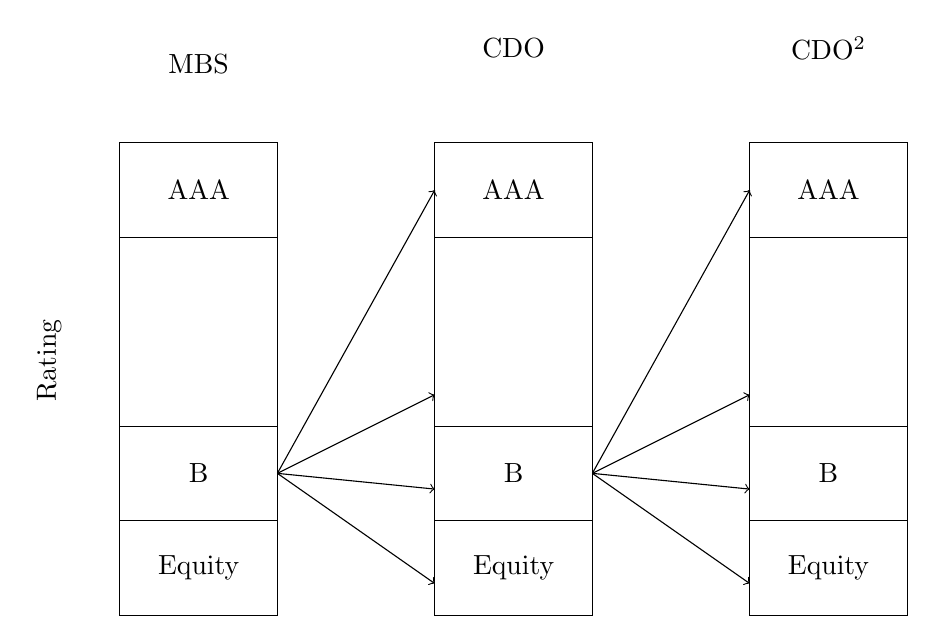
\begin{tikzpicture}[xscale=20,yscale=20]
\draw (0.0, .06) rectangle (0.1, 0);
\draw (0.0, .12) rectangle (0.1, .06);
\draw (0.0, .24) rectangle (0.1, .12);
\draw (0.0, .30) rectangle (0.1, .24);
\node  at (0.05,.35) {MBS};
\node  at (0.05,.27) {AAA};
\node  at (0.05,.09) {B};
\node  at (0.05,.03) {Equity};
\draw[->] (0.1,0.09) -- (.2,.27);
\draw[->] (0.1,0.09) -- (.2,.14);
\draw[->] (0.1,0.09) -- (.2,.08);
\draw[->] (0.1,0.09) -- (.2,.02);
\draw (0.2, .06) rectangle (.3, 0);
\draw (0.2, .12) rectangle (.3, .06);
\draw (0.2, .24) rectangle (.3, .12);
\draw (0.2, .30) rectangle (.3, .24);
\node  at (0.25,.36) {CDO};
\node  at (0.25,.27) {AAA};
\node  at (0.25,.09) {B};
\node  at (0.25,.03) {Equity};
\draw[->] (0.3,0.09) -- (.4,.27);
\draw[->] (0.3,0.09) -- (.4,.14);
\draw[->] (0.3,0.09) -- (.4,.08);
\draw[->] (0.3,0.09) -- (.4,.02);
\draw (0.4, .06) rectangle (.5, 0);
\draw (0.4, .12) rectangle (.5, .06);
\draw (0.4, .24) rectangle (.5, .12);
\draw (0.4, .30) rectangle (.5, .24);
\node  at (0.45,.36) {CDO$^2$};
\node  at (0.45,.27) {AAA};
\node  at (0.45,.09) {B};
\node  at (0.45,.03) {Equity};
\node[label=below:\rotatebox{90}{Rating}] at (-0.045,0.2) {};
\end{tikzpicture}
\caption{Multiple rounds of ABS}
\label{fig:mbs}
\end{figure}

\subsubsection{Example}

Consider the case where $X=\left\{a,b,c,d\right\}$ and the probability of a state going back to itself is close to one and uniform otherwise. Hence, the system spends a quarter of the time in each state. The interest rate is assumed to be constant. The collection of theories in the market is given by $\mathbf{F}=\left\{\mathcal{A},\mathcal{B},\mathcal{C}\right\}$, where
\begin{eqnarray*}
\mathcal{A} & = & \left\{\left\{a,d\right\},\left\{b,c\right\}\right\} \\
\mathcal{B} & = & \left\{\left\{a,b,d\right\},\left\{c\right\}\right\} \\
\mathcal{C} & = & \left\{\left\{a,b,c,d\right\}\right\}
\end{eqnarray*}
All theories in the market achieve statistical consistency: the perceived transition probability for agent $\mathcal{A}$ from states $a$ or $d$ to states $a$ or $d$ tends to one half, the perceived transition probability for agent $\mathcal{B}$ from states $a$, $b$ or $d$ to states $a$, $b$ or $d$ tends to one third and the perceived transition probability for agent $\mathcal{C}$ from any state to any other tends to one fourth.

For this example, it can be shown that a tranching that is issuer-optimal is one where there are four tranches and the attachment points coincide with the realizations of the asset price. Let $q$ be the waterfall equilibrium price function for the issuer-optimal tranching. Assume that the dividend function is such that $q(a)>q(b)>q(c)>q(d)$. In order of seniority, the tranches are labeled $s$ (senior), $m$ (mezzanine), $j$ (junior) and $e$ (equity). Table \ref{tab:ptr} presents the payoff function for each tranche.

\begin{table}
\caption{Security payoffs for the issuer-optimal tranching}
\label{tab:ptr}
\centering
\begin{tabular}{crrrrc}
\hline
States & \multicolumn{1}{c}{$\phi_e$} & \multicolumn{1}{c}{$\phi_j$} & \multicolumn{1}{c}{$\phi_m$} & \multicolumn{1}{c}{$\phi_s$} \\
\hline
$~~a$ & $q(a)-q(b)$             & $q(b)-q(c)$ & $q(c)-q(d)$ & $q(d)$ \\
$~~b$ & \multicolumn{1}{c}{$0$} & $q(b)-q(c)$ & $q(c)-q(d)$ & $q(d)$ \\
$~~c$ & \multicolumn{1}{c}{$0$} & \multicolumn{1}{c}{$0$} & $q(c)-q(d)$ & $q(d)$ \\
$~~d$ & \multicolumn{1}{c}{$0$} & \multicolumn{1}{c}{$0$} & \multicolumn{1}{c}{$0$} & $q(d)$ \\
 \hline
\end{tabular}
\end{table}

In state $d$, theory $\mathcal{A}$ buys the tranche $e$,  theory $\mathcal{B}$ buys the tranche $j$ and  theory $\mathcal{C}$ buys the tranche $m$. All agents have the same willingness to pay regarding tranche $s$. In state $d$, three different types of agents have claims on the underlying asset.

Instead of a unique round of securitization with four tranches, consider three rounds of securitization. In the first round, the underlying asset is securitized into debt and equity tranches. In the second round, the debt tranche of the first round is securitized into other debt and equity tranches. In the third round, the debt tranche of the second round is securitized into more debt and equity tranches (Figure \ref{fig:tree}). Let $\phi^i_e$ and $\phi^i_f$ be the payoffs from the equity and the debt tranches in the $i$-th round of securitization, where $i\in\left\{1,2,3\right\}$. Table \ref{tab:pit} shows the assumed payoff for each tranche. By construction, the payoff from the debt and the equity tranches add up to the payoff from the debt tranche from the previous round.

\begin{figure}[h]
\centering
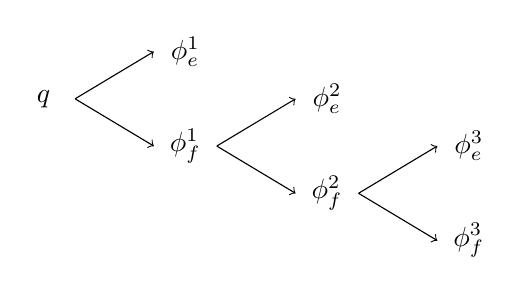
\begin{tikzpicture}[xscale=20,yscale=20]
\node[align=left]  at (0.03,0.25) {$q$};
\draw[->] (0.05,0.25) -- (.1,.28);
\draw[->] (0.05,0.25) -- (.1,.22);
\node[align=right]  at (.12,.28) {$\phi^1_e$};
\node[align=right]  at (.12,.22) {$\phi^1_f$};
\draw[->] (0.14,0.22) -- (.19,.25);
\draw[->] (0.14,0.22) -- (.19,.19);
\node[align=right]  at (.21,.25) {$\phi^2_e$};
\node[align=right]  at (.21,.19) {$\phi^2_f$};
\draw[->] (0.23,0.19) -- (.28,.22);
\draw[->] (0.23,0.19) -- (.28,.16);
\node[align=right]  at (.30,.22) {$\phi^3_e$};
\node[align=right]  at (.30,.16) {$\phi^3_f$};
\end{tikzpicture}
\caption{Iterated securitization}
\label{fig:tree}
\end{figure}

\begin{table}
\caption{Security payoffs for the iterated case}
\label{tab:pit}
\centering
\begin{tabular}{ c | c c | c c | c c }
\hline
States & $\phi^1_e$ & $\phi^1_f$ & $\phi^2_e$ & $\phi^2_f$ & $\phi^3_e$ & $\phi^3_f$ \\
\hline
$a$ & $q(a)-q(b)$ & $q(b)$ & $q(b)-q(c)$ & $q(c)$ & $q(c)-q(d)$ & $q(d)$ \\
$b$ & $0$         & $q(b)$ & $q(b)-q(c)$ & $q(c)$ & $q(c)-q(d)$ & $q(d)$ \\
$c$ & $0$         & $q(c)$ & $0$         & $q(c)$ & $q(c)-q(d)$ & $q(d)$ \\
$d$ & $0$         & $q(d)$ & $0$         & $q(d)$ & $0$         & $q(d)$ \\
 \hline
\end{tabular}
\end{table}

Consider the equilibrium in state $d$. The equity tranche of the 1st round will be bought by theory $\mathcal{A}$, the equity tranche of the 2nd round will be bought by theory $\mathcal{B}$, and the equity tranche of the 3rd round will be bought by theory $\mathcal{C}$. The value of the debt tranche on the 3rd round will be $q(d)$, discounted by the interest rate. Given this and the willingness to pay by agent $\mathcal{C}$ on the equity tranche of the 3rd round, the value of the debt tranche in the 2nd round will be $q(d)$ plus three quarters of $q(c)-q(d)$, discounted by the interest rate. Given this and the willingness to pay by agent $\mathcal{B}$ on the equity tranche of the 2nd round, the value of the debt tranche in the 1st round will be $q(d)$ plus three quarters of $q(c)-q(d)$ plus two thirds of $q(b)-q(c)$, discounted by the interest rate. Given this and the willingness to pay by agent $\mathcal{A}$ on the equity tranche of the 1st round, the value of the asset at state $d$ will be the dividend at $d$ plus $q(d)$ plus three quarters of $q(c)-q(d)$ plus two thirds of $q(b)-q(c)$ plus half of $q(a)-q(c)$, discounted by the interest rate. This is the same asset price equation for the aforementioned case of one round of securitization with four tranches.

A way of reading the equilibrium transactions at state $d$ is that agent $\mathcal{A}$ is borrowing from agent $\mathcal{B}$ using the underlying asset as collateral. In turn, agent $\mathcal{B}$ is borrowing from agent $\mathcal{C}$ using the debt issued by $\mathcal{A}$ as collateral. The equilibrium features a \textit{pyramiding arrangement}, as defined by \cite{Geanakoplos1996}.

\subsubsection{General case}

In order to define what will be labeled an \textit{iterated securitization equilibrium}, consider the following structure. Let there be a tree where $\mathbb{N}$ is its finite set of nodes, $r\in\mathbb{N}$ is its root node and $\mathbb{Z}\subset\mathbb{N}$ is its set of terminal nodes. Let $a:\mathbb{N}\setminus\left\{r\right\}\to\mathbb{N}\setminus\mathbb{Z}$ be a function where $a(n)$ denotes the predecessor of $n$. The root node $r$ represents the long-term asset. Each node $n\in\mathbb{N}\setminus\left\{r\right\}$ represents a security backed by asset $a(n)$. Nodes in $\mathbb{Z}$ represent securities that are not further securitized.

For $m\in\mathbb{N}\setminus\mathbb{Z}$, denote by $S(m)$ the set of $m$'s successors:
\[
S(m) = \left\{ n \in \mathbb{N}\setminus \left\{r\right\} : a(n)=m \right\}
\]

Let $(\tau_n)_{n\in\mathbb{N}}$ be a collection of intervals such that
\begin{enumerate}
\item $\tau_r=[0,\infty)$ and
\item for $m\in\mathbb{N}\setminus\mathbb{Z}$, the collection $(\tau_n)_{n\in S(m)}$ partitions the interval \[[0,\sup(\tau_{m})-\inf(\tau_{m})]\]
\end{enumerate}

Each security in $\mathbb{N}\setminus\left\{r\right\}$ is a straddle with a maturity of one period. Its payoff is a function of the cash flow from its predecessor. Specifically, if $t$ is the cash flow from asset $a(n)$, then the cash flow for security $n\in\mathbb{N}\setminus\left\{r\right\}$ would be given by:
\begin{equation} \label{eq:psi}
\zeta_n(t) = (t-\inf(\tau_n))^+ - (t-\sup(\tau_n))^+
\end{equation}
Hence, for $m\in\mathbb{N}\setminus\mathbb{Z}$:
\begin{equation*}
\zeta_{m}(t) = \sum_{n\in S(m)}\zeta_{n}(t)
\end{equation*}
This confirms that the cash flow from securities in $S(m)$ add up to the cash flow from asset $m$.

Let $\gamma_n:X\to\mathbb{R}_+$ be the cash flow for security $n\in\mathbb{N}$ as a function of the state of the world. If $q:X\to\mathbb{R}_+$ is the price function for the long-term asset, then $\gamma_r=q$  and
\begin{equation} \label{eq:gamma}
\gamma_{n}(x) = \zeta_n(\gamma_{a(n)}(x))
\end{equation}
for $n\in\mathbb{N}\setminus\left\{r\right\}$ and $x\in X$.

A tuple $\Sigma=\left(\mathbb{N},r,\mathbb{Z},a,(\tau_n)_{n\in\mathbb{N}}\right)$ is labeled an \textit{iterated securitization structure}.

\begin{dfn} \label{def:ise}
For a given iterated securitization structure $\Sigma$, an iterated securitization equilibrium is a function $p_{\Sigma}:\mathbb{N}\times X \to \mathbb{R}_+$ such that, for $x\in X$,
\begin{enumerate}
\item
\begin{equation} \label{eq:pr}
p_{\Sigma}(r,x) = \frac{d(x)}{R(x)}+\sum_{n\in S(r)}p_{\Sigma}(n,x)
\end{equation}
\item For $m\in\mathbb{N}\setminus(\mathbb{Z}\cup\left\{r\right\})$,
\begin{equation} \label{eq:pm}
p_{\Sigma}(m,x) = \sum_{n\in S(m)}p_{\Sigma}(n,x)
\end{equation}
\item For $z\in\mathbb{Z}$,
\begin{equation} \label{eq:pz}
p_{\Sigma}(z,x) = \frac{\max_{\mathcal{F}\in\mathbf{F}}E_{\mathcal{F}}\left(\gamma_z\mid x\right)}{R(x)}
\end{equation}
where $\gamma_r=p_{\Sigma}(r,\cdot)$ and, for $n\in\mathbb{N}\setminus\left\{r\right\}$, $\gamma_n$ is given by equation (\ref{eq:gamma}).
\end{enumerate}
\end{dfn}

The function $p_{\Sigma}(r,\cdot)$ is the price function for the long-term asset. Equation (\ref{eq:pr}) states that it is given by the discounted declared dividend plus the added prices of the securities derived from it. Equation (\ref{eq:pm}) states that for the securities that are not terminal nodes, their price is given by the added prices of the securities derived from them. Finally, equation (\ref{eq:pz}) gives the equilibrium for the terminal nodes, i.e. the securities that are not further securitized. Their price is given by the highest expectation regarding the cash flow coming from them. Ultimately, the cash flow from the securities at the terminal nodes will depend on the price of the long-term asset in the next period.

\begin{prp} \label{thm:equiv}
For any iterated securitization structure $\Sigma$, there is a tranching $\mathcal{T}$ such that
\begin{equation*}
p_{\Sigma}(r,x)= q_{\mathcal{T}}(x)
\end{equation*}
for $x\in X$
\end{prp}

\textsc{Proof:} See the proof of Proposition \ref{thm:equiv} below.

Proposition \ref{thm:equiv} states the equivalence between the equilibrium concepts in Definitions \ref{def:core} and \ref{def:ise}. For any iterated securitization equilibrium, the price of the long-term asset is the same as in a waterfall equilibrium for a suitable tranching $\mathcal{T}$. Intuitively, multiple rounds of securitization are redundant since the same outcome can be obtained by tranching the long-term asset into $|\mathbb{Z}|$ securities in a single round.

\subsection{Return example with three theories}\label{app:return-example}

This appendix provides the example summarized in Subsection \ref{sec:ep}, in which securitization can increase a theory's excess return even though that excess return remains negative. Consider a state space $X =\left\{l,m,h\right\}$ where the probability of a state going back to itself is close to one and uniform otherwise. The collection of theories is $\mathbf{F}=\left\{\mathcal{A},\mathcal{B},\mathcal{C}\right\}$, where:
\begin{eqnarray*}
\mathcal{A} & = &
\left\{
\left\{l\right\},
\left\{m,h\right\}
\right\},
\\
\mathcal{B} & = &
\left\{
\left\{l,h\right\},
\left\{m\right\}
\right\},
\\
\mathcal{C} & = &
\left\{
\left\{l,m,h\right\}
\right\}.
\end{eqnarray*}
The interest rate is constant and the dividend is such that, in the benchmark equilibrium, $q(l) < q(m) <q(h)$.

\begin{table}[h]
\caption{Expected payoffs from the long-term asset in the benchmark}
\label{tab:lastw}
\centering
\begin{tabular}{ c | c  |  c c c | c   }
\hline
States & $T(\psi)$ & $E_\mathcal{A}(\psi)$ & $E_\mathcal{B}(\psi)$ & $E_\mathcal{C}(\psi)$ & $\mathbf{B}$ \\
\hline
$l$ & $q(l)$ & $q(l)$ & $\frac{1}{2}\left(q(l)+q(h)\right)$ & $\frac{1}{3}\left(q(l)+q(m)+q(h)\right)$ & $\left\{\mathcal{B}\right\}$ \\
$m$ & $q(m)$ & $\frac{1}{2}\left(q(m)+q(h)\right)$ & $q(m)$ & $\frac{1}{3}\left(q(l)+q(m)+q(h)\right)$ & $\left\{\mathcal{A}\right\}$  \\
$h$ & $q(h)$         & $\frac{1}{2}\left(q(m)+q(h)\right)$ & $\frac{1}{2}\left(q(l)+q(h)\right)$ & $\frac{1}{3}\left(q(l)+q(m)+q(h)\right)$         & $\left\{\mathcal{A}\right\}$  \\
 \hline
\end{tabular}
\end{table}

Consider the case without any ABS. Table \ref{tab:lastw} presents i) the true expected price $T(\psi)$, ii) the expected price by each agent and, given these, iii) the set $\mathbf{B}$ of agents who will buy the long-term asset. All these objects are functions of the state of the world. If the dividend at state $h$ is high enough, the asset is bought by $\mathcal{B}$ at state $l$ and by $\mathcal{A}$ at states $m$ and $h$. Agent $\mathcal{C}$, who is less sophisticated than the other two, has a ``loser's blessing'' that allows him to have a non-negative excess return:
\[\underline{\Delta}_\mathcal{A}=-\frac{1}{6}\left(q(h)-q(m)\right) + \frac{1}{6}\left(q(h)-q(m)\right)=0\]
\[\underline{\Delta}_\mathcal{B}=-\frac{1}{6}\left(q(h)-q(l)\right)<0\]
\[\underline{\Delta}_\mathcal{C}=0\]

Consider now the case where ABS are introduced. A collection of three tranches with attachment points $0$, $q(l)$ and $q(m)$ is an issuer-optimal tranching if $q$ is its waterfall equilibrium and $q(l) < q(m) < q(h)$. The most senior tranche pays $q(l)$ at every state so there is no excess return from it. The excess returns for the mezzanine and the junior tranches can be obtained from Tables \ref{tab:lastm} and \ref{tab:laste}, respectively. These tables present i) the actual expected payoffs $T(\psi_\tau)$, ii) the expected payoff for each agent and, given these, iii) the set $\mathbf{B}(\tau,\cdot)$ of buyers for each of these tranches.

\begin{table}[h]
\caption{Expected payoffs from the mezzanine tranche}
\label{tab:lastm}
\centering
\begin{tabular}{ c | c  |  c c c | c   }
\hline
States & $T(\psi_m)$ & $E_\mathcal{A}(\psi_m)$ & $E_\mathcal{B}(\psi_m)$ & $E_\mathcal{C}(\psi_m)$ & $\mathbf{B}(m,\cdot)$ \\
\hline
$l$ & $0$ & $0$ & $\frac{1}{2}\left(q(m)-q(l)\right)$ & $\frac{2}{3}\left(q(m)-q(l)\right)$ & $\left\{\mathcal{C}\right\}$ \\
$m$ & $q(m)-q(l)$ & $q(m)-q(l)$ & $q(m)-q(l)$ & $\frac{2}{3}\left(q(m)-q(l)\right)$ & $\left\{\mathcal{A}\right\}$  \\
$h$ & $q(m)-q(l)$         & $q(m)-q(l)$ & $\frac{1}{2}\left(q(m)-q(l)\right)$ & $\frac{2}{3}\left(q(m)-q(l)\right)$         & $\left\{\mathcal{A}\right\}$  \\
 \hline
\end{tabular}
\end{table}

\begin{table}[h]
\caption{Expected payoffs from the junior tranche}
\label{tab:laste}
\centering
\begin{tabular}{ c | c  |  c c c | c   }
\hline
States & $T(\psi_j)$ & $E_\mathcal{A}(\psi_j)$ & $E_\mathcal{B}(\psi_j)$ & $E_\mathcal{C}(\psi_j)$ & $\mathbf{B}(j,\cdot)$ \\
\hline
$l$ & $0$ & $0$ & $\frac{1}{2}\left(q(h)-q(m)\right)$ & $\frac{1}{3}\left(q(h)-q(m)\right)$ & $\left\{\mathcal{B}\right\}$ \\
$m$ & $0$ & $\frac{1}{2}\left(q(h)-q(m)\right)$ & $0$ & $\frac{1}{3}\left(q(h)-q(m)\right)$ & $\left\{\mathcal{A}\right\}$  \\
$h$ & $q(h)-q(m)$         & $\frac{1}{2}\left(q(h)-q(m)\right)$ & $\frac{1}{2}\left(q(h)-q(m)\right)$ & $\frac{1}{3}\left(q(h)-q(m)\right)$         & $\left\{\mathcal{A}\right\}$  \\
 \hline
\end{tabular}
\end{table}

Thanks to the introduction of ABS, $\mathcal{C}$ is lured into buying the mezzanine tranche at state $l$. As a consequence, $\mathcal{C}$'s return with securitization is lower than without. Meanwhile, at the expense of agent $\mathcal{C}$, the excess return for $\mathcal{B}$ is higher than what it would be without securitization, even though it remains negative:
\[\Delta_\mathcal{A}=0=\underline{\Delta}_\mathcal{A}\]
\[\Delta_\mathcal{B}=-\frac{1}{6}\left(q(h)-q(m)\right)>\underline{\Delta}_\mathcal{B}\]
\[\Delta_\mathcal{C}=-\frac{2}{9}\left(q(m)-q(l)\right)<\underline{\Delta}_\mathcal{C}\]
Thanks to the introduction of ABS, some agents manage to get rid of toxic assets and increase their portfolio return.

\subsection{Proofs}

\textsc{Proof of Lemma \ref{refine}}:
Since $\mathcal{S}$ is a refinement of $\mathcal{T}$, for any function $g:X\to\mathbb{R}_{+}$ and any $x\in X$, the following  inequality holds:

\begin{eqnarray*}
\sum_{\tau\in\mathcal{T}}\max_{\mathcal{F}\in\mathbf{F}}E_{\mathcal{F}}
\left(\phi_\tau\left(g\right)\right)(x)
\leq
\sum_{\upsilon\in\mathcal{S}}\max_{\mathcal{F}\in\mathbf{F}}E_{\mathcal{F}}
\left(\phi_{\upsilon}\left(g\right)\right)(x)
\end{eqnarray*}
\\
Hence $\Psi_{\mathcal{T}}(g)(x)\leq \Psi_\mathcal{S}(g)(x)$ and so $q_\mathcal{T}(x)\leq \Psi_\mathcal{S}(q_\mathcal{T})(x)$.

Let $\Psi_\mathcal{S}^n$ denote the $n$-fold iterate of $\Psi_\mathcal{S}$. Since $\Psi_\mathcal{S}$ is monotone (see the proof of Proposition \ref{exu}), induction gives
\[
q_\mathcal{T}(x)\leq \Psi_\mathcal{S}^{n}(q_\mathcal{T})(x)
\]
for all $x\in X$ and all $n\geq 1$. Since $\Psi_\mathcal{S}$ is a contraction and $q_\mathcal{S}$ is its unique fixed point, $\Psi_\mathcal{S}^{n}(q_\mathcal{T})$ converges to $q_\mathcal{S}$. Therefore $q_\mathcal{T}(x)\leq q_\mathcal{S}(x)$ for all $x\in X$.

\hfill $\Box$

Definition \ref{def:dom} and Lemmas \ref{Urefine}, \ref{prp:Ucon} and \ref{prp:nUcon} will be used to prove Proposition \ref{mthm}.

\begin{dfn} \label{def:dom}
A tranching $\mathcal{T}$ satisfies the dominance condition if, for each  $\tau\in\mathcal{T}$ and $x\in X$, there is a theory $\mathcal{G}\in\mathbf{F}$ such that
\begin{equation*}
G^{\mathcal{T}}_
{\mathcal{G}}
\left(t\mid x\right)
\leq
G^{\mathcal{T}}_
{\mathcal{F}}
\left(t\mid x\right)
\end{equation*}
for $d\phi_\tau$-almost every $t\in\tau$ and all $\mathcal{F}\in\mathbf{F}$.
\end{dfn}

\begin{lmm} \label{Urefine}
If $\mathcal{T}$ satisfies the dominance condition and $\mathcal{S}$ is a refinement of $\mathcal{T}$, then $q_{\mathcal{S}}= q_{\mathcal{T}}$.
\end{lmm}

\begin{proof}
For $q=q_{\mathcal{T}}$, the payoff from a bounded tranche $\tau$ expected for next period by theory $\mathcal{F}$ on state $x$ can be written as
\begin{eqnarray}
E_{\mathcal{F}}
\left( \phi_\tau \left( q \right) \right)
(x) & = &
\int_{\inf(\tau)}^{\sup(\tau)}
\phi_\tau \left( t \right)
dG^\mathcal{T}_{\mathcal{F}}\left(t\mid x\right)
+
\int_{\sup(\tau)}^{\infty}
\phi_\tau \left( t \right)
dG^\mathcal{T}_{\mathcal{F}}\left(t\mid x\right)
\\ & = &
\sup(\tau)-\inf(\tau)
-\int_{\inf(\tau)}^{\sup(\tau)}
G^\mathcal{T}_{\mathcal{F}}\left(t\mid x\right)d\phi_\tau(t) \label{eq:core}
\end{eqnarray}
If $\tau$ is unbounded, the same expression is obtained by truncating the upper limit at any $M>\max_{x\in X}q_{\mathcal{T}}(x)$; this is without loss because $X$ is finite.

Therefore, if $\mathcal{T}$ satisfies the dominance condition and $\mathcal{S}$ is a refinement of $\mathcal{T}$, then
\begin{eqnarray*}
\sum_{\upsilon \in \mathcal{S} : \upsilon\subset \tau}
\max_{\mathcal{F}\in\mathbf{F}}
E_{\mathcal{F}}
\left( \phi_{\upsilon} \left(q_{\mathcal{T}} \right)
\right)
(x)
& = &
\max_{\mathcal{F}\in\mathbf{F}}
E_{\mathcal{F}}
\left(
\sum_{\upsilon \in \mathcal{S} : \upsilon\subset \tau}
\phi_{\upsilon} \left(q_{\mathcal{T}} \right)
\right)
(x)
\\
& = &
\max_{\mathcal{F}\in\mathbf{F}}
E_{\mathcal{F}}
\left(
\phi_{\tau} \left(q_{\mathcal{T}} \right)
\right)
(x)
\end{eqnarray*}
for any $\tau\in\mathcal{T}$ and $x\in X$. Using equations (\ref{tpayoff}) and (\ref{eq:map}), it follows that
\begin{eqnarray*}
\Psi_{\mathcal{S} }
\left(q_{\mathcal{T} }\right) & = &
\Psi_{\mathcal{T} }
\left(q_{\mathcal{T} }\right) \\ & = &
q_{\mathcal{T} }
\end{eqnarray*}
\end{proof}

\begin{lmm} \label{prp:Ucon}
If $\mathcal{T}$ satisfies the dominance condition, then
\begin{equation*}
q_{\mathcal{S}}(x)\leq q_{\mathcal{T}}(x)
\end{equation*}
for all $x\in X$ and any tranching $\mathcal{S}$.
\end{lmm}

\begin{proof}
Let $\mathcal{S}\vee\mathcal{T}$ be the coarsest common refinement between $\mathcal{T}$ and $\mathcal{S}$.
By Lemma \ref{refine},
\begin{equation*}
q_{\mathcal{S}}(x) \leq q_{\mathcal{S}\vee\mathcal{T}}(x)
\end{equation*}
for $x\in X$.
By Lemma \ref{Urefine},
\begin{equation*}
q_{\mathcal{S}\vee\mathcal{T}}(x)= q_{\mathcal{T}}(x)
\end{equation*}
for $x\in X$.
\end{proof}

\begin{lmm} \label{prp:nUcon}
If $\mathcal{T}$ does not satisfy the dominance condition, then there is a tranching $\mathcal{S}$ such that
\begin{equation*}
q_{\mathcal{T}}(x)<q_{\mathcal{S}}(x)
\end{equation*}
for all $x\in X$.
\end{lmm}

\begin{proof}
Since $\mathcal{T}$ does not satisfy the dominance condition, there is a state $x\in X$ and a tranche $\tau\in\mathcal{T}$ for which no single theory minimizes $G^\mathcal{T}_{\mathcal{F}}(\cdot\mid x)$ on the active part of the tranche. Because $\mathbf{F}$ and $X$ are finite, the perceived distribution functions are step functions. Hence a refinement can split $\tau$ into subintervals on which different theories minimize the relevant integral, so that
\begin{eqnarray*}
\min_{\mathcal{F}\in\mathbf{F}}\int_{\inf(\tau)}^{\sup(\tau)}
G^{\mathcal{T}}_{\mathcal{F}}\left(t\mid x\right)d\phi_\tau(t) & > &
\min_{\mathcal{F}\in\mathbf{F}}\int_{\inf(\tau)}^{\inf(\upsilon)}
G^{\mathcal{T}}_{\mathcal{F}}\left(t\mid x\right)d\phi_\tau(t) \\ & + &
\min_{\mathcal{F}\in\mathbf{F}}\int_{\inf(\upsilon)}^{\sup(\upsilon)}
G^{\mathcal{T}}_{\mathcal{F}}\left(t\mid x\right)d\phi_\tau(t)  \\ & + &
\min_{\mathcal{F}\in\mathbf{F}}\int_{\sup(\upsilon)}^{\sup(\tau)}
G^{\mathcal{T}}_{\mathcal{F}}\left(t\mid x\right)d\phi_\tau(t)
\end{eqnarray*}
for some $\upsilon\subset\tau$. Let $\mathcal{S}$ be a refinement of $\mathcal{T}$ such that $\upsilon\in\mathcal{S}$. From equations (\ref{eq:map}) and (\ref{eq:core}), it then follows that
\begin{equation*}
\Psi_{\mathcal{T}}\left(q_{\mathcal{T}}\right)(x)  <  \Psi_{\mathcal{S}}\left(q_{\mathcal{T}}\right)(x)
\end{equation*}
Since $\mathcal{S}$ is a refinement of $\mathcal{T}$, the same argument used in the proof of Lemma \ref{refine} gives $q_{\mathcal{T}}\leq \Psi_\mathcal{S}(q_{\mathcal{T}})$, with strict inequality at state $x$. Iterating $\Psi_\mathcal{S}$ from $q_{\mathcal{T}}$ and using monotonicity and contraction convergence implies
\begin{equation}
q_{\mathcal{T}}(y)\leq q_{\mathcal{S}}(y)
\end{equation}
for all $y\in X$, with strict inequality for $y=x$. To see that the inequality is strict in every state, note that the strict increase from $q_{\mathcal{T}}(x)$ to $q_{\mathcal{S}}(x)$ raises at least one tranche payoff at state $x$. Since every theory assigns positive probability to a transition from any state to any other state, the price of that tranche is strictly higher at every current state. Therefore $q_{\mathcal{T}}(y)<q_{\mathcal{S}}(y)$ for every $y\in X$.
\end{proof}

\textsc{Proof of Proposition \ref{mthm}}: Follows directly from Definition \ref{def:dom} and Lemmas \ref{prp:Ucon} and \ref{prp:nUcon}.

\hfill $\Box$

\textsc{Proof of Proposition \ref{thm:equiv}}: From equations (\ref{eq:pr}), (\ref{eq:pm}) and (\ref{eq:pz}), it follows that

\begin{equation} \label{eq:pru}
p_{\Sigma}(r,x) = \frac{d(x)}{R(x)}+\sum_{z\in \mathbb{Z}}\frac{\max_{\mathcal{F}\in\mathbf{F}}E_{\mathcal{F}}\left(\gamma_z\mid x\right)}{R(x)}
\end{equation}
for $x\in X$.

Let $b(z)$ be the set of non-terminal nodes on the branch from $r$ to the predecessor of $z\in\mathbb{Z}$. Since $\gamma_r=p_{\Sigma}(r,\cdot)$, equations (\ref{eq:psi}) and (\ref{eq:gamma}) imply
\begin{eqnarray} \label{eq:gzx}
\gamma_z(x)  & = &
\left(p_{\Sigma}(r,x) - \sum_{n\in b(z)}\inf(\tau_n) - \inf(\tau_z) \right)^+ \\ \nonumber
& - &
\left(p_{\Sigma}(r,x) - \sum_{n\in b(z)}\inf(\tau_n) - \sup(\tau_z) \right)^+
\end{eqnarray}

for $x\in X$.

By replacing (\ref{eq:gzx}) into (\ref{eq:pru}) and using the equilibrium concept in Definition \ref{def:core}, it follows that $p_{\Sigma}(r,\cdot)=q_{\mathcal{T}}$
if the attachment points for tranching $\mathcal{T}$ are given by
\begin{equation*}
\left(\sum_{n\in b(z)}\inf(\tau_n) + \inf(\tau_z) \right)_{z\in\mathbb{Z}}
\end{equation*}

\hfill $\Box$





\bibliographystyle{plainnat}
\bibliography{Bibliography}

\end{document}
